\documentclass[aspectratio=169,10pt]{beamer}

% ==============================================================================
% Beamer Speaker Notes Toggle (Swapped via `make notes` for dual-screen cue cards)
% ==============================================================================
\usepackage{pgfpages}
\setbeameroption{hide notes}

% ==============================================================================
% Modern Minimalist Beamer Theme for MLOps Architecture Defence
% ==============================================================================
\usetheme{default}
\useinnertheme{rectangles}
\usefonttheme{structurebold}

\usepackage[utf8]{inputenc}
\usepackage{tgheros}
\usepackage{microtype}
\renewcommand{\familydefault}{\sfdefault}

\usepackage{graphicx}
\usepackage{booktabs}
\usepackage{array}
\usepackage{ragged2e}
\usepackage{amsmath}
\usepackage{amssymb}
\usepackage{tikz}
\usetikzlibrary{shapes.geometric,arrows.meta,positioning,fit,calc,backgrounds,shadows.blur}
\usepackage{xcolor}
\usepackage[most]{tcolorbox}
\newcommand{\toollogo}[1]{\raisebox{-0.18\height}{\includegraphics[height=1.05em]{logos/#1.png}}\,}

% --- Modern Professional Colour Palette ---
\definecolor{SlateDark}{HTML}{0F172A}    % Primary dark slate header
\definecolor{SlateMid}{HTML}{1E293B}     % Card border / secondary
\definecolor{SlateLight}{HTML}{F8FAFC}   % Card background fill
\definecolor{BlueAccent}{HTML}{2563EB}   % Engineering blue
\definecolor{GreenAccent}{HTML}{059669}  % Emerald verification / pass
\definecolor{AmberAccent}{HTML}{D97706}  % Amber telemetry / alert
\definecolor{RoseAccent}{HTML}{E11D48}   % Rose gatekeeper / reject
\definecolor{PurpleAccent}{HTML}{7C3AED} % Purple active learning / conformal
\definecolor{TealAccent}{HTML}{0D9488}   % Teal data engineering
\definecolor{TextMain}{HTML}{1E293B}     % Primary text
\definecolor{TextMuted}{HTML}{94A3B8}    % Secondary muted text

% --- Beamer Colour Mappings ---
\setbeamercolor{normal text}{fg=TextMain,bg=white}
\setbeamercolor{structure}{fg=BlueAccent}
\setbeamercolor{frametitle}{fg=white,bg=SlateDark}
\setbeamercolor{title}{fg=white,bg=SlateDark}
\setbeamercolor{block title}{fg=white,bg=BlueAccent}
\setbeamercolor{block body}{fg=TextMain,bg=SlateLight}

% --- Clean Header / Footer Templates ---
\setbeamertemplate{navigation symbols}{}
\setbeamertemplate{headline}{}

\setbeamertemplate{frametitle}{%
    \nointerlineskip
    \begin{beamercolorbox}[wd=\paperwidth,ht=30pt,dp=8pt,leftskip=14pt,rightskip=14pt]{frametitle}
        \begin{minipage}[c][30pt][c]{0.50\textwidth}
            \raggedright
            \vspace*{-2.0pt}%
            {\large\bfseries\color{white}\insertframetitle}
        \end{minipage}%
        \hfill
        \begin{minipage}[c][30pt][c]{0.47\textwidth}
            \raggedright
            \vspace*{2.0pt}%
            \ifx\insertframesubtitle\@empty\else
                {\footnotesize\color{TextMuted}\insertframesubtitle}
            \fi
        \end{minipage}
    \end{beamercolorbox}
}

\setbeamertemplate{footline}{%
    \begin{beamercolorbox}[wd=\paperwidth,ht=12pt,dp=3pt,leftskip=14pt,rightskip=14pt]{normal text}
        {\tiny\color{TextMuted!90}\textbf{TaxonVision-MLOps} $\cdot$ MLOps Architecture (\texttt{main} Reference)}
        \hfill
        {\tiny\color{TextMuted!90}\insertframenumber{} / \inserttotalframenumber}
    \end{beamercolorbox}
}

% --- Clean Speaker Note Page Template & Readability Helpers ---
\newcommand{\cuetime}[1]{%
    \tcbox[on line, arc=2pt, colback=SlateDark, colframe=SlateDark, boxrule=0pt, left=4pt, right=4pt, top=1.5pt, bottom=1.5pt]{\tiny\bfseries\color{white}#1}%
}
\newcommand{\cuejury}[1]{%
    \begin{tcolorbox}[enhanced, colback=AmberAccent!10, colframe=AmberAccent!60, boxrule=0.4pt, arc=2pt, left=4pt, right=4pt, top=2.5pt, bottom=2.5pt, before skip=3pt, after skip=3pt]
        \scriptsize\textbf{\color{AmberAccent} Jury Q\&A:} #1
    \end{tcolorbox}%
}
\newcommand{\cueterms}[1]{%
    \vfill
    \vspace{2pt}
    {\color{SlateMid!35}\hrule height 0.4pt}
    \vspace{2pt}
    {\tiny\color{SlateMid!90}\textbf{Glossary:} #1}%
}
\setbeamertemplate{note page}{%
    \vbox to 0.91\paperheight{%
        \vskip 6pt
        {\footnotesize\bfseries\color{BlueAccent} Speaker Cue Card $\cdot$ Slide \insertframenumber: \insertframetitle}\\[2pt]
        {\tiny\color{SlateMid} \insertsubtitle}
        \vspace{2pt}
        {\color{BlueAccent!50}\hrule height 0.6pt}
        \vskip 5pt
        \setlength{\parskip}{2pt}
        {\scriptsize\color{TextMain}\insertnote}
        \vfil
    }%
}

% --- Custom tcolorbox Card Environments ---
\newtcolorbox{card}[1][]{
    enhanced, colback=SlateLight, colframe=SlateMid!30,
    boxrule=0.5pt, arc=2.5pt, left=5pt, right=5pt, top=3.5pt, bottom=3.5pt,
    fontupper=\scriptsize\RaggedRight,
    fuzzy shadow={0.6pt}{-0.6pt}{0pt}{0.1pt}{black!6}, #1
}
\newtcolorbox{bluecard}[1][]{
    enhanced, colback=BlueAccent!5, colframe=BlueAccent!60,
    boxrule=0.5pt, arc=2.5pt, left=5pt, right=5pt, top=3.5pt, bottom=3.5pt,
    fontupper=\scriptsize\RaggedRight,
    fuzzy shadow={0.6pt}{-0.6pt}{0pt}{0.1pt}{black!6}, #1
}
\newtcolorbox{greencard}[1][]{
    enhanced, colback=GreenAccent!5, colframe=GreenAccent!60,
    boxrule=0.5pt, arc=2.5pt, left=5pt, right=5pt, top=3.5pt, bottom=3.5pt,
    fontupper=\scriptsize\RaggedRight,
    fuzzy shadow={0.6pt}{-0.6pt}{0pt}{0.1pt}{black!6}, #1
}
\newtcolorbox{ambercard}[1][]{
    enhanced, colback=AmberAccent!5, colframe=AmberAccent!60,
    boxrule=0.5pt, arc=2.5pt, left=5pt, right=5pt, top=3.5pt, bottom=3.5pt,
    fontupper=\scriptsize\RaggedRight,
    fuzzy shadow={0.6pt}{-0.6pt}{0pt}{0.1pt}{black!6}, #1
}
\newtcolorbox{rosecard}[1][]{
    enhanced, colback=RoseAccent!5, colframe=RoseAccent!60,
    boxrule=0.5pt, arc=2.5pt, left=5pt, right=5pt, top=3.5pt, bottom=3.5pt,
    fontupper=\scriptsize\RaggedRight,
    fuzzy shadow={0.6pt}{-0.6pt}{0pt}{0.1pt}{black!6}, #1
}
\newtcolorbox{purplecard}[1][]{
    enhanced, colback=PurpleAccent!5, colframe=PurpleAccent!60,
    boxrule=0.5pt, arc=2.5pt, left=5pt, right=5pt, top=3.5pt, bottom=3.5pt,
    fontupper=\scriptsize\RaggedRight,
    fuzzy shadow={0.6pt}{-0.6pt}{0pt}{0.1pt}{black!6}, #1
}

% Stat Box Macro
\newcommand{\statbox}[3]{%
    \begin{tcolorbox}[enhanced, colback=#1!6, colframe=#1!60, boxrule=0.6pt, arc=3pt, left=3pt, right=3pt, top=3.5pt, bottom=3.5pt]
        \centering
        {\normalsize\bfseries\color{#1} #2}\\[1pt]
        {\tiny\textbf{\color{SlateMid} #3}}
    \end{tcolorbox}%
}

% --- Custom TikZ Component Styles ---
\tikzset{
    flowarrow/.style={-{Stealth[scale=0.75, length=3.6pt, width=2.8pt]}, line width=0.75pt, draw=SlateDark!75},
    dasharrow/.style={flowarrow, dashed, draw=BlueAccent},
    retrainarrow/.style={flowarrow, draw=RoseAccent, line width=0.85pt},
    syncarrow/.style={flowarrow, draw=GreenAccent, line width=0.85pt},
    passarrow/.style={flowarrow, draw=GreenAccent, line width=0.85pt},
    pill/.style={
        rectangle, rounded corners=2.5pt, fill=white, draw=SlateMid!40,
        inner sep=2.8pt, font=\tiny\bfseries, align=flush center
    },
    nodecard/.style={
        rectangle, rounded corners=2.5pt, draw=SlateMid!45, fill=SlateLight,
        line width=0.6pt, inner sep=3.5pt, align=flush center, font=\tiny
    },
    sysbox/.style={
        rectangle, rounded corners=2.5pt, draw=SlateMid!40, fill=white,
        line width=0.55pt, inner sep=3pt, align=flush center, font=\tiny
    },
    groupbox/.style={
        rectangle, rounded corners=3.5pt, line width=0.6pt, inner sep=4pt
    }
}

% --- Title Metadata ---
\title{\textbf{TaxonVision-MLOps}}
\subtitle{iNaturalist Species Classification with Safe Uncertainty \& Continuous Retraining}
\author{\textbf{Benjamin F\"orster}}
\institute{Liora Advanced Data Science \& MLOps Curriculum $\cdot$ Project Defence}
\date{November 2026}

\begin{document}

% ==============================================================================
% SLIDE 1: Title Slide (0:00 - 0:45)
% ==============================================================================
\begin{frame}[plain]
    \vspace{0.25cm}
    \begin{center}
        {\Huge\bfseries\color{SlateDark} TaxonVision-MLOps}\\[4pt]
        {\large\bfseries\color{BlueAccent} iNaturalist Species Classification with Safe Uncertainty \& Continuous Retraining}\\[10pt]

        \resizebox{0.98\textwidth}{!}{%
        \begin{tikzpicture}[node distance=0.22cm]
            \node[pill, fill=BlueAccent!10, draw=BlueAccent, minimum width=2.05cm] (p1) {\textbf{iNaturalist S3}\\{\tiny On-Demand Stream}};
            \node[pill, fill=TealAccent!10, draw=TealAccent, minimum width=2.05cm, right=of p1] (p2) {\textbf{\toollogo{dvc}8-Stage DVC DAG}\\{\tiny Epistemic Diamond}};
            \node[pill, fill=BlueAccent!12, draw=BlueAccent, minimum width=2.05cm, right=of p2] (p2b) {\textbf{\toollogo{mlflow}MLflow 3.x}\\{\tiny 4-Gate \texttt{@Production}}};
            \node[pill, fill=GreenAccent!10, draw=GreenAccent, minimum width=2.05cm, right=of p2b] (p3) {\textbf{\toollogo{onnx}INT8 ONNX API}\\{\tiny Conformal + Energy}};
            \node[pill, fill=AmberAccent!10, draw=AmberAccent, minimum width=2.05cm, right=of p3] (p4) {\textbf{\toollogo{grafana}17-Panel Cockpit}\\{\tiny \toollogo{evidently}$W_1$ \& $\text{MMD}_u^2$ Drift}};
            \node[pill, fill=PurpleAccent!10, draw=PurpleAccent, minimum width=2.05cm, right=of p4] (p5) {\textbf{\toollogo{airflow}Airflow 3 \& \toollogo{jenkins}Jenkins}\\{\tiny 7-Stage GPU CI/CD}};
            \draw[flowarrow] (p1) -- (p2);
            \draw[flowarrow] (p2) -- (p2b);
            \draw[flowarrow] (p2b) -- (p3);
            \draw[flowarrow] (p3) -- (p4);
            \draw[flowarrow] (p4) -- (p5);
        \end{tikzpicture}%
        }

        \vspace{0.35cm}
        \begin{columns}[T]
            \begin{column}{0.23\textwidth}
                \statbox{BlueAccent}{54.08 ms p95}{CPU INT8 (SLO $\le 350\text{ ms}$)}
            \end{column}
            \begin{column}{0.23\textwidth}
                \statbox{GreenAccent}{$\ge 95\%$ Target}{Split Conformal Coverage}
            \end{column}
            \begin{column}{0.23\textwidth}
                \statbox{PurpleAccent}{8 Stages}{DVC Epistemic Diamond}
            \end{column}
            \begin{column}{0.23\textwidth}
                \statbox{AmberAccent}{17 Panels}{2 Grafana Dashboards}
            \end{column}
        \end{columns}

        \vspace{0.30cm}
        {\small\textbf{Benjamin F\"orster}}\\[2pt]
        {\scriptsize\color{TextMuted!95} Reference Branch: \texttt{main} (Production \texttt{:30080}) $\cdot$ Integration: \texttt{develop} (Staging \texttt{:30085})}\\[2pt]
        {\scriptsize\color{TextMuted!95} 15 min Architecture Presentation + 5 min Live Cluster Demonstration}
    \end{center}
    \note{
        \textbf{Time: 0:00-0:45 (45s)}
        \begin{itemize}
            \item Good morning/afternoon. I am presenting \textbf{TaxonVision-MLOps} - a production-hardened computer vision platform for biological species identification (with \texttt{main} as the reference production branch and \texttt{develop} feeding staging).
            \item Rather than stopping at an isolated Jupyter prototype, we engineered a self-monitoring MLOps system on bare-metal Kubernetes (\texttt{k3s}): \textbf{54.08 ms} CPU ONNX p95 latency well inside our \textbf{350 ms} SLO, distribution-free \textbf{95\%} target conformal coverage, an \textbf{8-stage DVC Diamond DAG} executed by a \textbf{7-stage Jenkins GPU pipeline}, and a \textbf{17-panel Grafana cockpit}.
            \item I will spend 15 minutes on architectural trade-offs and safety guarantees, followed by a 5-minute live demonstration across the cluster and DagsHub.
        \end{itemize}
    }
\end{frame}

% ==============================================================================
% SLIDE 2: Introduction - Global Context, Goal & Core Stack
% ==============================================================================
\begin{frame}{Project Context \& Goal}{iNaturalist Brief: Production Chain First}
    \begin{columns}[c]
        \begin{column}{0.48\textwidth}
            \begin{card}
                \textbf{\color{BlueAccent} Global Context: iNaturalist \& Open Data}\\[2pt]
                \textbullet\ \textbf{Scale \& Licences:} \textbf{iNaturalist} hosts \textbf{270M+} observations (\textbf{170M} research-grade); only open AWS licences (\texttt{CC0}/\texttt{CC-BY}/\texttt{CC-BY-NC}) with attribution are usable.\\[2pt]
                \textbullet\ \textbf{Design Principle:} Separate immutable feature extraction (\texttt{timm} DINOv3) from fast-iterating decision boundaries (Class-Balanced head + conformal calibration) for low-cost, drift-responsive MLOps.
            \end{card}
            \vspace{0.05cm}
            \begin{greencard}
                \textbf{\color{GreenAccent} Project Goal (Levels 1-4 Achieved)}\\[2pt]
                \textbullet\ \textbf{1. Safe Serving:} Species + confidence (\textbf{54 ms} CPU) + CAM explanation, routing uncertain/OOD photos to \textbf{human review}.\\[2pt]
                \textbullet\ \textbf{2. Full Lineage:} Licence filtering, attribution, data/model versioning, and cost-latency benchmarking.\\[2pt]
                \textbullet\ \textbf{3. Closed Loop:} Drift checks, active learning, and automated retraining gated by 4 promotion checks.
            \end{greencard}
        \end{column}
        \begin{column}{0.49\textwidth}
            \begin{bluecard}
                \textbf{\color{SlateDark} Core MLOps Toolchain at a Glance}\\[3pt]
                \textbf{\color{TealAccent} Data \& Reproducibility:}\\[1.5pt]
                \toollogo{dvc}\textbf{DVC} $\cdot$ \toollogo{postgresql}\textbf{Postgres 16} $\cdot$ \toollogo{seaweedfs}\mbox{\textbf{SeaweedFS S3}} $\cdot$ \toollogo{dagshub}\textbf{DagsHub}\\[3pt]
                \textbf{\color{BlueAccent} Modelling, HPO \& Registry:}\\[1.5pt]
                \toollogo{pytorch}\textbf{PyTorch} $\cdot$ \toollogo{onnx}\textbf{ONNX INT8} $\cdot$ \toollogo{optuna}\textbf{Optuna} $\cdot$ \toollogo{mlflow}\textbf{MLflow 3.x}\\[3pt]
                \textbf{\color{PurpleAccent} Serving \& Infrastructure:}\\[1.5pt]
                \toollogo{fastapi}\textbf{FastAPI} $\cdot$ \toollogo{redis}\textbf{Redis} $\cdot$ \toollogo{docker}\textbf{Docker} $\cdot$ \toollogo{kubernetes}\textbf{Kubernetes (k3s)}\\[3pt]
                \textbf{\color{AmberAccent} Monitoring \& Automation:}\\[1.5pt]
                \toollogo{prometheus}\textbf{Prometheus} $\cdot$ \toollogo{grafana}\textbf{Grafana} $\cdot$ \toollogo{evidently}\textbf{Evidently}\\[1.5pt]
                \toollogo{airflow}\textbf{Airflow 3} $\cdot$ \toollogo{jenkins}\textbf{Jenkins} $\cdot$ \toollogo{githubactions}\textbf{GitHub Actions}
            \end{bluecard}
            \vspace{0.05cm}
            \begin{card}
                \centering\scriptsize
                \textbf{15-Minute Roadmap:} Problem $\to$ Architecture $\to$ Data \& Training $\to$ Safe Serving $\to$ Drift \& Closed-Loop Automation $\to$ \textbf{5-Min Live Demo}
            \end{card}
        \end{column}
    \end{columns}

    \note{
        \textbf{Time: 0:45-1:30 (45s)}
        \begin{itemize}
            \item Grounding this in the original project brief: \textbf{iNaturalist} hosts over 270M wildlife observations (around 170M research-grade), but only open-licensed AWS dataset images with preserved photographer attribution can legally enter training.
            \item Our design principle separates immutable feature extraction (\texttt{timm} DINOv3) from fast-iterating decision boundaries (Class-Balanced head + conformal calibration) for low-cost, drift-responsive MLOps.
            \item Our goal covers all four difficulty levels: fast \textbf{ONNX} inference with calibrated confidence, visual CAM explanations and human review referral for uncertain/OOD photos, strict open-licence lineage (\textbf{DVC} + \textbf{MLflow}), and a closed feedback loop (\textbf{Prometheus}, \textbf{Grafana}, \textbf{Evidently}, \textbf{Airflow 3}, \textbf{Jenkins}).
        \end{itemize}
    }
\end{frame}

% ==============================================================================
% SLIDE 3: Domain Challenge & Dual-Pipeline Strategy (1:30 - 2:30)
% ==============================================================================
\begin{frame}{Concept \& Dual-Pipeline Strategy}{Resilient Long-Tail Vision \& Roadmap Split}
    \begin{columns}[T]
        \begin{column}{0.33\textwidth}
            \begin{tcolorbox}[enhanced, colback=white, colframe=SlateMid!30, boxrule=0.5pt, arc=2.5pt, left=4pt, right=4pt, top=3pt, bottom=3pt]
                \centering\textbf{\tiny 1. Extreme Long-Tail Imbalance}\\[2pt]
                \resizebox{0.96\linewidth}{!}{%
                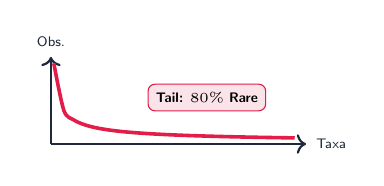
\begin{tikzpicture}[x=0.036cm, y=0.82cm]
                    \draw[->, thick, color=SlateMid] (0,0) -- (90,0) node[right, font=\tiny] {Taxa};
                    \draw[->, thick, color=SlateMid] (0,0) -- (0,1.35) node[above, font=\tiny] {Obs.};
                    \draw[smooth, domain=1:86, color=RoseAccent, line width=1.3pt] plot (\x, {1.25 / (\x^0.58)});
                    \node[pill, fill=RoseAccent!12, draw=RoseAccent] at (55, 0.72) {Tail: $80\%$ Rare};
                \end{tikzpicture}%
                }
            \end{tcolorbox}
            \vspace{0.1cm}
            \begin{rosecard}
                \textbf{\color{RoseAccent} 2. Softmax Hallucinations}\\
                $\sum \pi_k = 1$ forces high confidence ($>98\%$) on blur or uncatalogued species.\\[3pt]
                \textbf{\color{AmberAccent} 3. Taxonomic Drift}\\
                Biologists continually \emph{split} or \emph{lump} taxa; retraining weights per edit does not scale.
            \end{rosecard}
        \end{column}
        \begin{column}{0.64\textwidth}
            \centering
            \vspace{0.05cm}
            \resizebox{\textwidth}{!}{%
            \begin{tikzpicture}[node distance=0.35cm]
                % Pipeline 1
                \node[sysbox, draw=BlueAccent, fill=BlueAccent!10, text width=3.8cm] (p1_in) at (0, 1.55) {
                    \textbf{\color{BlueAccent} \toollogo{dvc}Pipeline 1: Weight-Centric}\\
                    {\tiny \textbf{[Live Production]} Offline DVC Diamond}
                };
                \node[sysbox, draw=BlueAccent!70, fill=white, text width=3.8cm] (p1_op) at (0, 0.35) {
                    \textbf{\toollogo{pytorch}Frozen DINOv3 ($D=384$)}\\
                    {\tiny Class-Balanced Head $\to$ \toollogo{onnx}INT8 ONNX}
                };

                % Pipeline 2
                \node[sysbox, draw=PurpleAccent, fill=PurpleAccent!10, text width=3.9cm] (p2_in) at (4.7, 1.55) {
                    \textbf{\color{PurpleAccent} Pipeline 2: Data-Centric}\\
                    {\tiny \textbf{[Strategy Roadmap]} Vision RAG \& MMKG}
                };
                \node[sysbox, draw=PurpleAccent!70, fill=white, text width=3.9cm] (p2_op) at (4.7, 0.35) {
                    \textbf{LanceDB HNSW + Metadata Store}\\
                    {\tiny $\mathcal{O}(1)$ Taxon Lumps/Splits $\cdot$ VLM Triage}
                };

                % Convergence
                \node[sysbox, draw=GreenAccent, fill=GreenAccent!12, text width=8.8cm] (serv) at (2.35, -0.95) {
                    \textbf{\color{GreenAccent} \toollogo{fastapi}FastAPI Serving Boundary (CPU \toollogo{onnx}INT8 ONNX: 54.08 ms p95 $\le 350\text{ ms}$ SLO)}\\
                    {\tiny Decisive ($|C|=1$): Auto-Accept \quad$\cdot$\quad Moderate ($2\le |C|\le 3$): Exemplar Context}\\
                    {\tiny Uncertain ($|C|=0$ or $|C|>3$): Route to Human Triage}
                };

                \draw[flowarrow, draw=BlueAccent] (p1_in) -- (p1_op);
                \draw[flowarrow, draw=PurpleAccent] (p2_in) -- (p2_op);
                \draw[passarrow] (p1_op.south) -- (p1_op.south |- serv.north) node[midway, left, font=\tiny\bfseries\color{BlueAccent}] {INT8 Graph + $\hat{q}$};
                \draw[dasharrow, draw=PurpleAccent] (p2_op.south) -- (p2_op.south |- serv.north) node[midway, right, font=\tiny\bfseries\color{PurpleAccent}] {Roadmap Extension};
            \end{tikzpicture}%
            }
            \vspace{0.1cm}
            \begin{card}
                \centering
                \textbf{\color{SlateDark} Operational Minimalism vs.\ Roadmap:} Production runs Pipeline 1's lightweight DINOv3 linear probe in deterministic INT8 ONNX (\texttt{CPUExecutionProvider}), whilst our Strategy Report specifies Pipeline 2's HNSW + knowledge-graph lookup for $\mathcal{O}(1)$ taxonomic splits/lumps without retraining.
            \end{card}
        \end{column}
    \end{columns}

    \note{
        \textbf{Time: 0:45-2:00 (1m 15s)}
        \begin{itemize}
            \item Why do standard vision classifiers fail on citizen-science photography? Three domain realities: an extreme long tail where 80\% of species are sparse, closed-world softmax forcing near-100\% confidence on camera blur or unseen phyla, and shifting taxonomic definitions.
            \item To avoid unnecessary neural bloat on the hot path, \textbf{Pipeline 1} - which is fully live in production - pairs a frozen \textbf{DINOv3 ViT-Small} foundation trunk with a convex Class-Balanced linear head exported to \textbf{INT8 ONNX} and guarded by Split Conformal and Helmholtz energy bounds.
            \item Looking ahead in our Strategy Report, \textbf{Pipeline 2} is cleanly decoupled as a future data-centric extension: vector retrieval (LanceDB HNSW) and metadata-driven taxonomic mapping handle sister-species disambiguation and taxonomic lumps/splits in $\mathcal{O}(1)$ edits without touching Pipeline 1 weights.
        \end{itemize}
    }
\end{frame}

% ==============================================================================
% SLIDE 3: End-to-End MLOps Architecture (2:00 - 3:20)
% ==============================================================================
\begin{frame}{End-to-End MLOps Architecture}{Ingress, Telemetry, Retraining \& Dual S3}
    \centering
    \vspace{-0.05cm}
    \resizebox{0.94\textwidth}{!}{%
    \begin{tikzpicture}[node distance=0.3cm]
        % --- 1. Edge Ingress & Dual-Tier Serving ---
        \node[sysbox, draw=BlueAccent, fill=BlueAccent!8, text width=2.2cm] (user) at (0, 1.55) {\textbf{Ecologist / User}\\{\tiny Web UI \& REST API}};
        \node[sysbox, draw=BlueAccent, fill=BlueAccent!12, text width=2.2cm] (trf) at (0, 0.50) {\textbf{Traefik v3.1}\\{\tiny Cloudflare Tunnel}};
        \node[sysbox, draw=TealAccent, fill=TealAccent!10, text width=2.2cm] (stg) at (-1.42, -0.75) {\textbf{Staging (\texttt{develop})}\\{\tiny \texttt{:30085} $\cdot$ 1 CPU Pod}};
        \node[sysbox, draw=BlueAccent, fill=BlueAccent!15, text width=2.2cm] (prd) at (1.42, -0.75) {\textbf{Prod (\texttt{main}, 2x)}\\{\tiny \texttt{:30080} $\cdot$ GPU Sliced}};
        \node[sysbox, draw=RoseAccent, fill=RoseAccent!10, text width=2.2cm] (red) at (-1.42, -2.05) {\textbf{\toollogo{redis}Redis Cache}\\{\tiny \texttt{taxon:img:*} SHA}};
        \node[sysbox, draw=BlueAccent!80, fill=white, text width=2.2cm] (htmx) at (1.42, -2.05) {\textbf{\toollogo{fastapi}HTMX Cockpit}\\{\tiny Forward CAM + Cards}};

        % --- 2. Observability, Logs & Drift Engine ---
        \node[sysbox, draw=AmberAccent, fill=AmberAccent!10, text width=2.55cm] (loki) at (5.00, 1.55) {\textbf{Promtail $\to$ Loki 3.0}\\{\tiny Structured JSON Logs}};
        \node[sysbox, draw=AmberAccent, fill=AmberAccent!10, text width=2.55cm] (prom) at (5.00, 0.50) {\textbf{\toollogo{prometheus}Prometheus (\texttt{:30090})}\\{\tiny Scrapes \texttt{/metrics} (15s)}};
        \node[sysbox, draw=AmberAccent, fill=AmberAccent!18, text width=2.55cm] (graf) at (5.00, -0.55) {\textbf{\toollogo{grafana}Grafana (\texttt{:30300})}\\{\tiny 17 Panels (2 Dashboards)}};
        \node[sysbox, draw=SlateDark, fill=SlateLight, text width=2.55cm] (pg) at (5.00, -1.60) {\textbf{\toollogo{postgresql}PostgreSQL 16}\\{\tiny 3 DBs (\texttt{telemetry} etc.)}};
        \node[sysbox, draw=AmberAccent!90, fill=white, text width=2.55cm] (evid) at (5.00, -2.60) {\textbf{\toollogo{evidently}Evidently UI (\texttt{:30082})}\\{\tiny 0.7 $W_1$ + $\text{MMD}_u^2$}};

        % --- 3. Active Learning & Retraining Loop ---
        \node[sysbox, draw=PurpleAccent, fill=PurpleAccent!12, text width=2.6cm] (ls) at (9.05, 1.30) {\textbf{\toollogo{dagshub}DagsHub Label Studio}\\{\tiny Expert Taxonomist Triage}};
        \node[sysbox, draw=AmberAccent!90, fill=AmberAccent!12, text width=2.6cm] (air_d) at (9.05, 0.05) {\textbf{\toollogo{airflow}Airflow Drift Monitor}\\{\tiny \texttt{@hourly} TaskFlow DAG}};
        \node[sysbox, draw=RoseAccent, fill=RoseAccent!12, text width=2.6cm] (air_r) at (9.05, -1.20) {\textbf{\toollogo{airflow}Airflow Retrain DAG}\\{\tiny \texttt{model\_retraining} (\texttt{:30095})}};
        \node[sysbox, draw=RoseAccent, fill=RoseAccent!18, text width=2.85cm] (jenk) at (9.05, -2.45) {\textbf{\toollogo{jenkins}On-Prem Jenkins (Docker)}\\{\tiny Ephemeral K3s GPU Pods}};

        % --- 4. In-Cluster NVMe Cache ---
        \node[sysbox, draw=PurpleAccent, fill=PurpleAccent!15, text width=2.6cm] (sea) at (12.90, 1.30) {\textbf{\toollogo{seaweedfs}Local SeaweedFS S3}\\{\tiny \texttt{taxon-dvc-cache} (NVMe)}};

        % --- 5. Managed Control Plane & Tracking (DagsHub) ---
        \node[sysbox, draw=GreenAccent, fill=GreenAccent!12, text width=2.6cm] (dvc) at (12.90, -0.15) {\textbf{\toollogo{dvc}DagsHub DVC Remote}\\{\tiny \texttt{s3://dvc} Public Archive}};
        \node[sysbox, draw=GreenAccent!80, fill=white, text width=2.6cm] (gha) at (12.90, -1.30) {\textbf{\toollogo{githubactions}GitHub Actions CI}\\{\tiny \texttt{dvc pull} (\texttt{DAGSHUB\_TOKEN})}};
        \node[sysbox, draw=GreenAccent, fill=GreenAccent!16, text width=2.6cm] (mlf) at (12.90, -2.45) {\textbf{\toollogo{mlflow}DagsHub MLflow 3.x}\\{\tiny Tracking \& Model Registry}};

        % Edges
        \draw[flowarrow] (user) -- (trf);
        \draw[flowarrow] (trf) -| (stg);
        \draw[flowarrow] (trf) -| (prd);
        \draw[flowarrow] (stg) -- (red);
        \draw[flowarrow] (prd) -- (red);
        \draw[flowarrow] (stg) -- (htmx);
        \draw[flowarrow] (prd) -- (htmx);

        \draw[dasharrow] (prd.east) -- ++(0.45,0) |- (loki.west);
        \draw[dasharrow] (prd.east) -- ++(0.45,0) |- (prom.west);
        \draw[flowarrow] (loki.east) -- ++(0.20,0) |- ([yshift=4pt]graf.east);
        \draw[flowarrow] (prom) -- (graf);
        \draw[dasharrow] (prd.east) -- ++(0.45,0) |- (pg.west);

        \draw[flowarrow] (pg.east) -- ++(0.32,0) |- (air_d.west);
        \draw[flowarrow] ([yshift=-4pt]air_d.west) -- ++(-0.35,0) |- (evid.east);
        \draw[retrainarrow] (air_d) -- (air_r) node[midway, fill=RoseAccent!3, inner sep=1pt, font=\tiny\bfseries\color{RoseAccent}] {Drift Alert};
        \draw[retrainarrow] ([yshift=-4pt]graf.east) -- ++(0.38,0) |- ([yshift=4pt]air_r.west);
        \draw[retrainarrow] (prd.east) -- ++(0.26,0) |- (3.10,-3.18) -- node[midway, below, font=\tiny\bfseries\color{RoseAccent}] {Flag Ambiguous / OOD} (7.05,-3.18) |- (ls.west);
        \draw[flowarrow] (ls.east) -- ++(0.20,0) |- ([yshift=-4pt]air_r.east);
        \draw[retrainarrow] (air_r) -- (jenk) node[midway, fill=RoseAccent!3, inner sep=1pt, font=\tiny\bfseries\color{RoseAccent}] {Headless GPU Job};

        \draw[syncarrow] (jenk.east) -- ++(0.25,0) |- (sea.west);
        \draw[syncarrow] (jenk.east) -- ++(0.25,0) |- (dvc.west);
        \draw[flowarrow] (gha) -- (dvc);
        \draw[syncarrow] (jenk) -- (mlf);
        \draw[dasharrow] (air_d.east) -- ++(0.35,0) |- ([yshift=4pt]mlf.west);

        % Subgraph Boxes
        \begin{scope}[on background layer]
            \node[groupbox, fill=BlueAccent!3, draw=BlueAccent!35, fit=(user)(trf)(stg)(prd)(red)(htmx), label={[font=\tiny\bfseries\color{BlueAccent}]above:1. Edge Ingress \& Dual-Tier Serving}] {};
            \node[groupbox, fill=AmberAccent!3, draw=AmberAccent!35, fit=(loki)(prom)(graf)(pg)(evid), label={[font=\tiny\bfseries\color{AmberAccent}]above:2. Telemetry, Logs \& Drift}] {};
            \node[groupbox, fill=RoseAccent!3, draw=RoseAccent!35, fit=(ls)(air_d)(air_r)(jenk), label={[font=\tiny\bfseries\color{RoseAccent}]above:3. Active Learning \& Retraining}] {};
            \node[groupbox, fill=PurpleAccent!3, draw=PurpleAccent!35, fit=(sea), label={[font=\tiny\bfseries\color{PurpleAccent}]above:4. NVMe Cache}] {};
            \node[groupbox, fill=GreenAccent!3, draw=GreenAccent!35, fit=(dvc)(gha)(mlf), label={[font=\tiny\bfseries\color{GreenAccent}]below:\toollogo{dagshub}5. Control Plane (DagsHub)}] {};
        \end{scope}
    \end{tikzpicture}%
    }
    \vspace{0.05cm}
    \begin{card}
        \centering\tiny
        \textbf{\color{BlueAccent} Goal $\to$ Takeaway:} Connect serving, telemetry, expert triage, and GPU retraining in one automated loop with zero manual handoffs.
    \end{card}
    \note{
        \begin{itemize}
            \item To answer directly how our components communicate: the system is partitioned into five cleanly isolated zones on \texttt{k3s} plus DagsHub.
            \item \textbf{1. Serving:} External traffic arrives over an outbound Cloudflare Tunnel to Traefik v3.1, routing \texttt{main} to 2 production replicas (\texttt{:30080}) and \texttt{develop} to a single CPU staging pod (\texttt{:30085}), sharing ephemeral Redis cache for cross-pod CAM heatmaps.
            \item \textbf{2. Telemetry:} FastAPI emits structured JSON logs (Promtail $\to$ Loki 3.0), exposes \texttt{/metrics} scraped every 15s by Prometheus (\texttt{:30090}) into Grafana (17 panels across 2 dashboards, \texttt{:30300}), and writes 384-D embeddings asynchronously to PostgreSQL 16.
            \item \textbf{3. Closed Loop:} Airflow's hourly monitor evaluates Wasserstein-1 and $\text{MMD}_u^2$ into Evidently UI (\texttt{:30082}) and DagsHub MLflow; OOD/ambiguous samples go to Label Studio; Grafana alerts or Drift DAGs trigger \texttt{model\_retraining}, which dispatches On-Prem Jenkins (Docker) to run ephemeral K3s GPU pods on the RTX 5070 Ti.
            \item \textbf{4 \& 5. Added Value of DagsHub:} Heavy cached embeddings sync locally over NVMe to SeaweedFS S3 (zero egress bills), whilst DagsHub acts as our unified public hub for Git, DVC (\texttt{s3://dvc}), MLflow 3.x Registry, and Label Studio under one \texttt{DAGSHUB\_TOKEN}.
        \end{itemize}
    }
\end{frame}

% ==============================================================================
% SLIDE 4: Data Plane & Database Consolidation (3:20 - 4:30)
% ==============================================================================
\begin{frame}{Data Plane \& DB Consolidation}{Open-Licence Filter, S3 Stream \& Postgres 16}
    \begin{columns}[T]
        \begin{column}{0.48\textwidth}
            \centering
            \textbf{\scriptsize\color{BlueAccent} Polars Parquet I/O \& On-Demand S3 Streamer}\\[3pt]
            \resizebox{\textwidth}{!}{%
            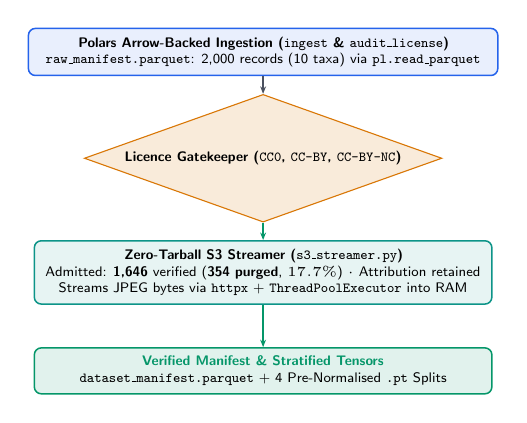
\begin{tikzpicture}
                \node[sysbox, draw=BlueAccent, fill=BlueAccent!10, text width=5.75cm] (pol) at (0, 2.75) {
                    \textbf{Polars Arrow-Backed Ingestion (\texttt{ingest} \& \texttt{audit\_license})}\\
                    {\tiny \texttt{raw\_manifest.parquet}: 2,000 records (10 taxa) via \texttt{pl.read\_parquet}}
                };
                \node[diamond, aspect=2.8, draw=AmberAccent, fill=AmberAccent!15, inner sep=2pt, font=\tiny\bfseries] (gate) at (0, 1.40) {
                    Licence Gatekeeper (\texttt{CC0}, \texttt{CC-BY}, \texttt{CC-BY-NC})
                };
                \node[sysbox, draw=TealAccent, fill=TealAccent!10, text width=5.6cm] (str) at (0, -0.05) {
                    \textbf{Zero-Tarball S3 Streamer (\texttt{s3\_streamer.py})}\\
                    {\tiny Admitted: \textbf{1,646} verified (\textbf{354 purged}, $17.7\%$) $\cdot$ Attribution retained}\\
                    {\tiny Streams JPEG bytes via \texttt{httpx} + \texttt{ThreadPoolExecutor} into RAM}
                };
                \node[sysbox, draw=GreenAccent, fill=GreenAccent!12, text width=5.6cm] (out) at (0, -1.30) {
                    \textbf{\color{GreenAccent} Verified Manifest \& Stratified Tensors}\\
                    {\tiny \texttt{dataset\_manifest.parquet} + 4 Pre-Normalised \texttt{.pt} Splits}
                };
                \draw[flowarrow] (pol) -- (gate);
                \draw[passarrow] (gate) -- (str);
                \draw[passarrow] (str) -- (out);
            \end{tikzpicture}%
            }
        \end{column}
        \begin{column}{0.49\textwidth}
            \centering
            \textbf{\scriptsize\color{GreenAccent} Database Evolution: Resolving k3s Lock Contention}\\[3pt]
            \resizebox{\textwidth}{!}{%
            \begin{tikzpicture}
                \node[sysbox, draw=RoseAccent!80, fill=RoseAccent!8, text width=5.6cm] (old) at (0, 2.45) {
                    \textbf{\color{RoseAccent} Prototype Persistence Bottleneck}\\
                    {\tiny Polars Parquet + Per-Service \textbf{SQLite WAL} Files}\\
                    {\tiny\color{RoseAccent} $\times$ Concurrent FastAPI telemetry, Optuna \& Airflow writes triggered \texttt{database is locked}}
                };
                \node[sysbox, draw=GreenAccent, fill=GreenAccent!12, text width=5.6cm] (pg) at (0, 0.85) {
                    \textbf{\color{GreenAccent} \toollogo{postgresql}Unified PostgreSQL 16 Cluster (\texttt{postgres:16-alpine})}\\
                    {\tiny UID \texttt{70} $\cdot$ \texttt{max\_connections=120} $\cdot$ Non-CoW NVMe (\texttt{chattr +C})}
                };
                \node[pill, fill=BlueAccent!12, draw=BlueAccent, text width=1.65cm] (db1) at (-1.9, -0.35) {\textbf{\toollogo{airflow}\texttt{airflow}}\\{\tiny DAG State}};
                \node[pill, fill=AmberAccent!12, draw=AmberAccent, text width=1.65cm] (db2) at (0, -0.35) {\textbf{\texttt{telemetry}}\\{\tiny 384-D Vectors}};
                \node[pill, fill=PurpleAccent!12, draw=PurpleAccent, text width=1.65cm] (db3) at (1.9, -0.35) {\textbf{\texttt{optuna}}\\{\tiny HPO Trials}};

                \node[sysbox, draw=SlateMid!50, fill=SlateLight, text width=5.6cm] (fb) at (0, -1.28) {
                    \textbf{Offline Resilience Invariant:} Graceful fallback to local \textbf{SQLite WAL} (\texttt{optuna\_studies.db}) \& bounded in-memory telemetry when \texttt{TAXON\_DATABASE\_URL} is unset.
                };

                \draw[passarrow] (old) -- (pg) node[midway, right, font=\tiny\bfseries\color{GreenAccent}] {Consolidated};
                \draw[flowarrow] (pg.south) -- (db1.north);
                \draw[flowarrow] (pg.south) -- (db2.north);
                \draw[flowarrow] (pg.south) -- (db3.north);
            \end{tikzpicture}%
            }
        \end{column}
    \end{columns}

    \note{
        \textbf{Time: 3:20-4:30 (1m 10s)}
        \begin{itemize}
            \item Two core data-engineering decisions prevented storage bloat and concurrency failures.
            \item On the left: Stage 1 pulls 2,000 DarwinCore records across 10 target species into \texttt{raw\_manifest.parquet}. Stage 2 (\texttt{audit\_license}) enforces Creative Commons compliance (\texttt{CC0}, \texttt{CC-BY}, \texttt{CC-BY-NC}) whilst preserving photographer attribution - purging 354 non-compliant records and leaving 1,646 verified observations. Stage 3 streams only those JPEGs on demand over HTTPS via \texttt{httpx} into RAM - zero multi-gigabyte image tarballs on disk.
            \item On the right: early SQLite WAL persistence broke under concurrent FastAPI workers, Optuna sweeps, and Airflow heartbeats with \texttt{database is locked} errors. We consolidated all three relational databases (\texttt{airflow}, \texttt{telemetry}, \texttt{optuna}) into one \texttt{postgres:16-alpine} cluster backed by a non-CoW NVMe directory (\texttt{chattr +C}) to prevent BTRFS block fragmentation.
        \end{itemize}
    }
\end{frame}

% ==============================================================================
% SLIDE 5: Tri-Plane Orchestration, Airflow DAGs & Jenkins CI/CD (4:30 - 5:45)
% ==============================================================================
\begin{frame}{Tri-Plane CI/CD Orchestration}{GitHub Actions, Airflow 3 \& 7-Stage Jenkins}
    \centering
    \resizebox{0.94\textwidth}{!}{%
    \begin{tikzpicture}
        % 3 Orchestration Planes
        \node[sysbox, draw=BlueAccent, fill=BlueAccent!8, text width=4.1cm] (gha) at (0, 2.0) {
            \textbf{\color{BlueAccent} \toollogo{githubactions}1. GitHub Actions (Cloud CPU)}\\
            {\tiny PR Gates: Ruff, MyPy (84 files), 306 Tests}\\
            {\tiny \textbf{DVC:} \texttt{dvc pull} $\cdot$ Publishes \texttt{ghcr.io/...:sha-<7>}}
        };
        \node[sysbox, draw=PurpleAccent, fill=PurpleAccent!8, text width=4.5cm] (air) at (4.7, 2.0) {
            \textbf{\color{PurpleAccent} \toollogo{airflow}2. Airflow 3 (\texttt{LocalExecutor}, \texttt{:30095})}\\
            {\tiny TaskFlow (\texttt{@dag}, \texttt{@task}, \texttt{@task.short\_circuit})}\\
            {\tiny UID \texttt{50000} $\cdot$ Zero CUDA in scheduler; REST control}
        };
        \node[sysbox, draw=RoseAccent, fill=RoseAccent!8, text width=4.55cm] (jen) at (9.65, 2.0) {
            \textbf{\color{RoseAccent} \toollogo{jenkins}3. On-Prem Jenkins (Docker $\to$ 7 Stages)}\\
            {\tiny Ephemeral K3s Pods (\texttt{ServiceAccount: jenkins-agent})}\\
            {\tiny \textbf{DVC:} Runs 8-stage \texttt{dvc repro} \& Dual \texttt{dvc push}}
        };

        % Airflow Two DAGs Box
        \node[sysbox, draw=PurpleAccent!70, fill=white, text width=6.4cm] (dag1) at (1.2, 0.55) {
            \textbf{\color{PurpleAccent} DAG 1: \texttt{prediction\_drift\_monitor} (\texttt{@hourly})}\\
            {\tiny \texttt{evaluate\_live\_drift} (POST \texttt{/drift/evaluate}) $\gg$ \texttt{is\_drift\_detected} (\texttt{short\_circuit}) $\gg$ \texttt{trigger\_retraining}}
        };
        \node[sysbox, draw=RoseAccent!70, fill=white, text width=6.7cm] (dag2) at (8.3, 0.55) {
            \textbf{\color{RoseAccent} DAG 2: \texttt{model\_retraining} (Event / Drift Triggered)}\\
            {\tiny \texttt{merge\_human\_feedback} (Label Studio) $\gg$ \texttt{trigger\_jenkins\_build} (CSRF) $\gg$ \texttt{wait\_for\_jenkins} $\gg$ \texttt{report\_promotion\_outcome}}
        };

        \draw[flowarrow, draw=PurpleAccent] (air.south) -- ++(0,-0.2) -| (dag1.north);
        \draw[flowarrow, draw=RoseAccent] (air.south) -- ++(0,-0.2) -| (dag2.north);
        \draw[retrainarrow] (dag1.east) -- (dag2.west);
        \draw[retrainarrow] (jen.south |- dag2.north) -- (jen.south);

        % 7 Jenkins Stages Bar
        \node[pill, fill=SlateLight, draw=SlateMid!50, text width=1.65cm] (j1) at (-1.15, -0.75) {\textbf{1. Prepare}\\{\tiny Pixi Toolchain}};
        \node[pill, fill=BlueAccent!10, draw=BlueAccent, text width=1.85cm] (j2) at (0.85, -0.75) {\textbf{2. Static Gates}\\{\tiny Lint/MyPy/OKF}};
        \node[pill, fill=BlueAccent!10, draw=BlueAccent, text width=1.65cm] (j3) at (2.85, -0.75) {\textbf{3. Unit Tests}\\{\tiny \texttt{tests/unit/} Suite}};
        \node[pill, fill=PurpleAccent!10, draw=PurpleAccent, text width=1.95cm] (j4) at (4.90, -0.75) {\textbf{4. Conformal}\\{\tiny Integr./Bounds ($\ge 80\%$)}};
        \node[pill, fill=TealAccent!10, draw=TealAccent, text width=1.65cm] (j5) at (6.95, -0.75) {\textbf{5. Strict Docs}\\{\tiny OKF/Zensical}};
        \node[pill, fill=RoseAccent!15, draw=RoseAccent, text width=2.05cm] (j6) at (9.05, -0.75) {\textbf{6. GPU Train}\\{\tiny 8-Stage DVC Repro}};
        \node[pill, fill=GreenAccent!15, draw=GreenAccent, text width=1.85cm] (j7) at (11.25, -0.75) {\textbf{7. K8s Deploy}\\{\tiny SHA Pin \& Smoke}};

        \draw[flowarrow] (j1) -- (j2);
        \draw[flowarrow] (j2) -- (j3);
        \draw[flowarrow] (j3) -- (j4);
        \draw[flowarrow] (j4) -- (j5);
        \draw[flowarrow] (j5) -- (j6);
        \draw[flowarrow] (j6) -- (j7);
    \end{tikzpicture}%
    }
    \vspace{0.15cm}
    \begin{card}
        \centering
        \textbf{\color{SlateDark} Stage 7 K3s Rollout:} Jenkins stages checkpoints atomically (\texttt{.tmp} $\to$ \texttt{mv -f}) onto NVMe \texttt{hostPath}, applies Kustomize (\texttt{main} $\to$ \texttt{taxon-vision}, \texttt{develop} $\to$ \texttt{taxon-vision-staging}), pins immutable \texttt{ghcr.io/...:sha-<7>}, waits up to \texttt{600s} rollout, and verifies via \texttt{verify\_deployment.sh}.
    \end{card}
    \note{
        \textbf{Time: 4:30-5:45 (1m 15s)}
        \begin{itemize}
            \item \textbf{Jury Question: What is Airflow's role, and which DAGs did you set up?}
            \item Notice the clean separation between cloud CI, workflow orchestration, and GPU execution:
            \item \textbf{GitHub Actions} guards every PR on CPU (Ruff, strict MyPy across 84 source files, 306 pytest cases) and builds immutable \texttt{:sha-<7>} containers to GHCR.
            \item \textbf{Apache Airflow 3 (\texttt{:30095})} holds zero CUDA weights - it orchestrates via REST:
                \begin{itemize}
                    \item \texttt{prediction\_drift\_monitor} (\texttt{@hourly}): queries \texttt{POST /api/v1/drift/evaluate}, short-circuits cleanly if clean, or fires retraining.
                    \item \texttt{model\_retraining}: merges verified Label Studio annotations, fetches a Jenkins CSRF crumb, dispatches the headless GPU build, polls status, and checks MLflow promotion.
                \end{itemize}
            \item \textbf{On-Prem Jenkins (Docker)} dispatches 7 top-level CI/CD stages into ephemeral K3s pods (CPU-only for Stages 1-5/7; RTX 5070 Ti GPU pod delegated solely for Stage 6), and Stage 7 rolls out Kustomize overlays safely.
        \end{itemize}
    }
\end{frame}

% ==============================================================================
% SLIDE 6: 8-Stage Epistemic Diamond DVC DAG (5:45 - 7:00)
% ==============================================================================
\begin{frame}{The 8-Stage DVC Diamond DAG}{Zero-Leakage Splits \& Dual-Remote Lineage}
    \begin{columns}[c]
        \begin{column}{0.68\textwidth}
            \centering
            \resizebox{\textwidth}{!}{%
            \begin{tikzpicture}
                % Row 1: Ingestion & Extraction
                \node[sysbox, draw=BlueAccent, fill=BlueAccent!10, text width=2.3cm] (a) at (0.2, 2.35) {
                    \textbf{1. \texttt{ingestion} (frozen)}\\{\tiny \texttt{pipelines.ingest}}\\{\tiny \texttt{raw\_manifest.parquet}}
                };
                \node[sysbox, draw=BlueAccent, fill=BlueAccent!10, text width=2.45cm] (b) at (3.2, 2.35) {
                    \textbf{2. \texttt{audit\_license}}\\{\tiny \texttt{pipelines.audit\_license}}\\{\tiny \texttt{dataset\_manifest.parquet}}
                };
                \node[sysbox, draw=BlueAccent, fill=BlueAccent!15, text width=2.55cm] (c) at (6.25, 2.35) {
                    \textbf{3. \texttt{extract\_features}}\\{\tiny \texttt{pipelines.extract\_features}}\\{\tiny DINOv3 (384-D Pre-Norm)}
                };

                % Row 2: 4 Stratified Split Tensors
                \node[pill, fill=GreenAccent!12, draw=GreenAccent, text width=1.95cm] (d1) at (-0.15, 1.00) {\textbf{70\% Train}\\{\tiny \texttt{train\_embeddings.pt}}};
                \node[pill, fill=GreenAccent!12, draw=GreenAccent, text width=1.95cm] (d2) at (2.75, 1.00) {\textbf{10\% Val}\\{\tiny \texttt{val\_embeddings.pt}}};
                \node[pill, fill=PurpleAccent!12, draw=PurpleAccent, text width=1.95cm] (d3) at (6.85, 1.00) {\textbf{10\% Cal (155)}\\{\tiny \texttt{cal\_embeddings.pt}}};
                \node[pill, fill=AmberAccent!12, draw=AmberAccent, text width=1.95cm] (d4) at (9.10, 1.00) {\textbf{10\% Test (164)}\\{\tiny \texttt{test\_embeddings.pt}}};

                % Row 3: Drift, Train, ONNX
                \node[sysbox, draw=AmberAccent, fill=AmberAccent!12, text width=2.08cm] (e) at (-0.15, -0.45) {
                    \textbf{4. \texttt{data\_drift}}\\{\tiny \texttt{pipelines.data\_drift}}\\{\tiny $W_1 + \text{MMD}^2$ vs Ref \texttt{.dvc}}
                };
                \node[sysbox, draw=BlueAccent, fill=BlueAccent!12, text width=2.05cm] (f) at (2.75, -0.45) {
                    \textbf{5. \texttt{train} (Head)}\\{\tiny \texttt{pipelines.train}}\\{\tiny Class-Balanced $\to$ \texttt{head.pt}}
                };
                \node[sysbox, draw=BlueAccent, fill=BlueAccent!12, text width=2.10cm] (g) at (5.38, -0.45) {
                    \textbf{6. \toollogo{onnx}\texttt{export} (ONNX)}\\{\tiny \texttt{pipelines.export\_onnx}}\\{\tiny INT8 PTQ (\texttt{model\_int8.onnx})}
                };

                % Row 4: Calibrate, Evaluate, Registry
                \node[sysbox, draw=PurpleAccent, fill=PurpleAccent!12, text width=2.35cm] (h) at (2.75, -1.90) {
                    \textbf{7. \texttt{calibrate}}\\{\tiny \texttt{pipelines.calibrate}}\\{\tiny \texttt{conformal\_config.yaml}}
                };
                \node[sysbox, draw=RoseAccent, fill=RoseAccent!12, text width=2.35cm] (i) at (5.75, -1.90) {
                    \textbf{8. \texttt{eval} (Pareto)}\\{\tiny \texttt{pipelines.evaluate}}\\{\tiny 4 Promotion Gates}
                };
                \node[sysbox, draw=GreenAccent, fill=GreenAccent!18, text width=2.2cm] (j) at (8.90, -1.90) {
                    \textbf{\texttt{@Production}}\\{\tiny \toollogo{mlflow}DagsHub MLflow 3.x}\\{\tiny + \texttt{model\_passport}}
                };

                % Connections (balanced lengths & clean orthogonal channels)
                \draw[flowarrow] (a) -- (b);
                \draw[flowarrow] (b) -- (c);
                \draw[flowarrow] (c.south) -- ++(0,-0.32) -| (d1.north);
                \draw[flowarrow] (c.south) -- ++(0,-0.32) -| (d2.north);
                \draw[flowarrow] (c.south) -- ++(0,-0.32) -| (d3.north);
                \draw[flowarrow] (c.south) -- ++(0,-0.32) -| (d4.north);

                \draw[flowarrow] (d1.south) -- (e.north);
                \draw[flowarrow] (d1.south) -- ++(0,-0.26) -| ([xshift=-14pt]f.north);
                \draw[flowarrow] (e) -- (f) node[midway, above, yshift=2pt, inner sep=1pt, font=\tiny\bfseries\color{SlateMid}] {Audit};
                \draw[flowarrow] ([xshift=6pt]d2.south) -- ([xshift=6pt]f.north);
                \draw[flowarrow] (f) -- (g);

                \draw[flowarrow] (g.south) -- ++(0,-0.25) -| ([xshift=-6pt]h.north);
                \draw[flowarrow] (d3.south) -- ++(0,-1.88) -| ([xshift=6pt]h.north);
                \draw[flowarrow] (h) -- (i);
                \draw[flowarrow] (g.south) -- ++(0,-0.25) -| ([xshift=-6pt]i.north);
                \draw[flowarrow] (d4.south) -- ++(0,-2.02) -| ([xshift=6pt]i.north);
                \draw[passarrow] (i) -- (j);
            \end{tikzpicture}%
            }
        \end{column}
        \begin{column}{0.30\textwidth}
            \begin{purplecard}[fontupper=\tiny\RaggedRight]
                \textbf{\scriptsize\color{PurpleAccent} \toollogo{seaweedfs}Local SeaweedFS S3}\\[1.5pt]
                \textbullet\ \texttt{dvc push -r local-seaweedfs}\\
                \textbullet\ Apache 2.0 (Haystack needle packing on NVMe).\\
                \textbullet\ Hosts \texttt{taxon-dvc-cache} \& \texttt{triage-queue} buckets.\\
                \textbullet\ Zero cloud egress bills.
            \end{purplecard}
            \vspace{0.05cm}
            \begin{greencard}[fontupper=\tiny\RaggedRight]
                \textbf{\scriptsize\color{GreenAccent} \toollogo{dvc}DagsHub S3 (\texttt{origin})}\\[1.5pt]
                \textbullet\ \texttt{dvc push -r origin}\\
                \textbullet\ Public cryptographic archive via \texttt{dvc.lock} MD5s.\\
                \textbullet\ CI pulls checkpoints using \texttt{DAGSHUB\_TOKEN} without cluster VPN access.
            \end{greencard}
        \end{column}
    \end{columns}
    \vspace{0.05cm}
    \begin{card}
        \centering\tiny
        \textbf{\color{TealAccent} Goal $\to$ Takeaway:} Isolate Cal/Test splits from Train/Val to prevent coverage leakage whilst tracking every artefact via MD5s.
    \end{card}
    \note{
        \textbf{Time: 5:45-7:00 (1m 15s)}
        \begin{itemize}
            \item \textbf{Jury Question: What versioning mechanisms do you apply to datasets, and what is the added value of DagsHub?}
            \item All data and model transformations run as pure stages in our \textbf{8-stage DVC Diamond DAG} (\texttt{dvc.yaml}), with every Parquet manifest and \texttt{.pt} tensor cryptographically hashed in \texttt{dvc.lock}. Note Stage 1 (\texttt{ingestion}) is marked \texttt{frozen: true} so \texttt{dvc repro} skips redundant API scraping unless explicitly refreshed.
            \item Crucially, Stage 3 partitions embeddings into four strict splits: \textbf{70\% Train}, \textbf{10\% Val}, \textbf{10\% Cal} ($n=155$), and \textbf{10\% Test} ($n=164$). Isolating \texttt{Val} (HPO early stopping) from \texttt{Cal} (conformal quantiles) prevents statistical coverage leakage.
            \item Stage 4 (\texttt{data\_drift}) audits training drift ($W_1 = 0.0107 < 0.1281$, $\text{MMD}^2$ $p=0.741$) prior to Stage 5 head fitting, Stage 6 INT8 ONNX export, Stage 7 conformal calibration, and Stage 8 4-gate promotion.
            \item Dual S3 Remotes: Heavy intermediates sync locally to SeaweedFS over NVMe, whilst release artefacts mirror to DagsHub S3 so GitHub Actions can test real ONNX weights in the cloud.
        \end{itemize}
    }
\end{frame}

% ==============================================================================
% SLIDE 7: Feature Caching, Optuna HPO & MLflow 3.x Registry (7:00 - 8:10)
% ==============================================================================
\begin{frame}{Training, Optuna \& MLflow 3.x}{Cached Features, CB Loss \& Zero Pollution}
    \centering
    \resizebox{0.94\textwidth}{!}{%
    \begin{tikzpicture}
        % Column 1: Feature Caching
        \node[sysbox, draw=BlueAccent, fill=BlueAccent!10, text width=3.5cm] (vit) at (0, 1.55) {
            \textbf{\color{BlueAccent} Frozen DINOv3 Trunk}\\
            {\tiny \texttt{vit\_small\_patch16\_dinov3.lvd1689m}}\\
            {\tiny Extracted \textbf{ONCE} ($D=384$) $\to$ \texttt{.pt}}
        };
        \node[sysbox, draw=TealAccent, fill=TealAccent!10, text width=3.5cm] (cb) at (0, -0.05) {
            \textbf{\color{TealAccent} Class-Balanced Linear Head}\\
            {\tiny $E_n = \frac{1-\beta^n}{1-\beta}$, Optuna $\beta = 0.9959$}\\
            {\tiny 30 Epochs in \textbf{2.63 s} ($92.68\%$ Val Acc)}
        };

        % Column 2: Optuna Bayesian HPO
        \node[sysbox, draw=PurpleAccent, fill=PurpleAccent!10, text width=3.9cm] (opt) at (4.55, 1.55) {
            \textbf{\color{PurpleAccent} \toollogo{optuna}Optuna TPE + ASHA Pruner}\\
            {\tiny 6D Space (\texttt{lr, wd, dropout, beta, bs, noise})}\\
            {\tiny \toollogo{postgresql}PostgreSQL \texttt{optuna} DB (\texttt{:30081})}
        };
        \node[sysbox, draw=RoseAccent!80, fill=RoseAccent!8, text width=1.8cm] (t_bad) at (3.5, -0.05) {
            \textbf{\color{RoseAccent} Weak Trials}\\
            {\tiny ASHA Pruned}\\
            {\tiny No Reg.\ Pollution}
        };
        \node[sysbox, draw=GreenAccent!80, fill=GreenAccent!10, text width=1.85cm] (t_good) at (5.6, -0.05) {
            \textbf{\color{GreenAccent} Persisted Best}\\
            {\tiny \texttt{best\_params.yaml}}\\
            {\tiny $\to$ \texttt{head.pt}}
        };

        % Column 3: MLflow 3.x & Model Passport
        \node[sysbox, draw=GreenAccent, fill=GreenAccent!12, text width=4.3cm] (mlf) at (9.55, 1.55) {
            \textbf{\color{GreenAccent} \toollogo{mlflow}DagsHub MLflow 3.x Continuity}\\
            {\tiny Single Parent Run (\texttt{resume\_parent\_mlflow\_run})}\\
            {\tiny 4-Split MD5s (\texttt{mlflow.data}) + PR/Energy Plots}
        };
        \node[sysbox, draw=SlateDark, fill=SlateLight, text width=4.3cm] (pass) at (9.55, -0.05) {
            \textbf{\color{SlateDark} Stage 8 Only Promotion}\\
            {\tiny Git SHA $\cdot$ DVC MD5 $\cdot$ $\hat{q}$ $\cdot$ $\tau_{\text{ood}}$ $\cdot$ 4-Gate Verdict}\\
            {\tiny Aliases: \texttt{@Production} / \texttt{@Challenger} / \texttt{@Archived}}
        };

        \draw[flowarrow] (vit) -- (cb);
        \draw[flowarrow] (cb.east) -- ++(0.3,0) |- (opt.west);
        \draw[retrainarrow] ([xshift=-4pt]opt.south) -- ++(0,-0.22) -| (t_bad.north);
        \draw[passarrow] ([xshift=4pt]opt.south) -- ++(0,-0.22) -| (t_good.north);
        \draw[passarrow] (t_good.east) -- ++(0.3,0) |- (mlf.west);
        \draw[flowarrow] (mlf) -- (pass);
    \end{tikzpicture}%
    }
    \vspace{0.15cm}
    \begin{columns}[T]
        \begin{column}{0.48\textwidth}
            \begin{bluecard}
                \textbf{\color{BlueAccent} Calibration-Damped Objective \& $\beta \in [0.99, 0.9999]$:}\\
                Objective divides peak val PR-AUC by $1 + \lambda \cdot \min(\text{val\_loss})$ to stop weight decay vanishing and logit saturation; $\beta = 0.9959$ preserves rare-taxa weighting without exploding gradients.
            \end{bluecard}
        \end{column}
        \begin{column}{0.48\textwidth}
            \begin{greencard}
                \textbf{\color{GreenAccent} Zero Registry Pollution Invariant:}\\
                Optuna trials log metrics in batches (\texttt{log\_batch()}) and are forbidden from registering models. Only Stage 8 (\texttt{evaluate.py}) updates \texttt{@Production} / \texttt{@Challenger} aliases on DagsHub MLflow.
            \end{greencard}
        \end{column}
    \end{columns}

    \note{
        \textbf{Time: 7:00-8:10 (1m 10s)}
        \begin{itemize}
            \item \textbf{Jury Questions: How is MLflow used to track experiments and manage models? What is your strategy to move a model to Production?}
            \item Because DINOv3 stays frozen, fitting the Dropout + Linear cosine head on cached tensors takes \textbf{2.63 seconds} for 30 epochs ($92.68\%$ validation accuracy).
            \item That speed lets Optuna (TPE sampler + ASHA pruner persisted in PostgreSQL, visualised on \texttt{:30081}) search our 6D regularised space, using a validation-loss-damped objective so search cannot strip L2 decay and inflate OOD softmax confidence.
            \item In \textbf{DagsHub MLflow 3.x}, Stage 5 opens one parent run and Stages 6-8 re-enter it via \texttt{resume\_parent\_mlflow\_run()}, attaching dataset MD5s (\texttt{mlflow.data}), confusion matrices, PR curves, and energy plots. Crucially, trials never pollute the Registry - only Stage 8's automated 4-gate check promotes models to \texttt{@Production} or stages them as \texttt{@Challenger}.
        \end{itemize}
    }
\end{frame}

% ==============================================================================
% SLIDE 8: Serving Topology, Startup Model Loading & Redis Cache (8:10 - 9:20)
% ==============================================================================
\begin{frame}{Serving Topology \& Redis Cache}{Startup Hydration, GPU Slicing \& CAM Cache}
    \begin{columns}[T]
        \begin{column}{0.31\textwidth}
            \statbox{GreenAccent}{54.08 ms}{CPU ONNX p95 ($\le 350\text{ ms}$ SLO)}
        \end{column}
        \begin{column}{0.31\textwidth}
            \statbox{BlueAccent}{91.46\%}{INT8 Top-1 ($0.9782$ Med AP)}
        \end{column}
        \begin{column}{0.31\textwidth}
            \statbox{PurpleAccent}{19.9 FPS}{CPU Throughput (p50: 49.02 ms)}
        \end{column}
    \end{columns}
    \vspace{0.12cm}
    \centering
    \resizebox{0.94\textwidth}{!}{%
    \begin{tikzpicture}
        % Ingress
        \node[sysbox, draw=SlateDark, fill=SlateLight, text width=3.1cm] (trf) at (0, 0.75) {
            \textbf{Traefik v3.1 Ingress}\\
            {\tiny Cloudflare \texttt{hive-mind-tunnel}}
        };

        % Staging Track
        \node[sysbox, draw=TealAccent, fill=TealAccent!10, text width=3.5cm] (stg) at (4.4, 1.95) {
            \textbf{\color{TealAccent} Staging (\texttt{:30085}, \texttt{develop})}\\
            {\tiny 1 Pod $\cdot$ \textbf{CPU-Only} (\texttt{0 GPU})}\\
            {\tiny Never starves Jenkins GPU runs}
        };

        % Production Track
        \node[sysbox, draw=BlueAccent, fill=BlueAccent!12, text width=3.5cm] (prd) at (4.4, 0.75) {
            \textbf{\color{BlueAccent} \toollogo{kubernetes}Prod (\texttt{:30080}, \texttt{main})}\\
            {\tiny 2 Replicas (\texttt{maxSurge:1, maxUnavail:0})}\\
            {\tiny 2x \texttt{nvidia.com/gpu} Time-Sliced}
        };

        % Canary Track
        \node[sysbox, draw=AmberAccent, fill=AmberAccent!10, text width=3.5cm] (can) at (4.4, -0.45) {
            \textbf{\color{AmberAccent} Canary A/B \texttt{[Manifest Ready]}}\\
            {\tiny \texttt{canary-ab-service.yaml} (80/20 split)}\\
            {\tiny Ready for \texttt{@Prod} / \texttt{@Challenger}}
        };

        % Right Column: Planarized Redis Cache (Top) + Startup ONNX (Bottom)
        \node[sysbox, draw=RoseAccent, fill=RoseAccent!10, text width=4.3cm] (red) at (9.5, 1.60) {
            \textbf{\color{RoseAccent} \toollogo{redis}Redis Ephemeral Cache (\texttt{redis:6379})}\\
            {\tiny \texttt{taxon:img:<sha256>} (15m TTL)}\\
            {\tiny Solves Multi-Pod Split-Brain for \texttt{/explain} CAM}
        };
        \node[sysbox, draw=GreenAccent, fill=GreenAccent!12, text width=4.3cm] (onnx) at (9.5, 0.15) {
            \textbf{\color{GreenAccent} \toollogo{onnx}Startup Model Hydration (\texttt{/health/ready})}\\
            {\tiny \texttt{lifespan} + \texttt{readinessProbe} warm \texttt{@lru\_cache} singletons}\\
            {\tiny Atomic \texttt{hostPath} (\texttt{ro}) $\cdot$ Zero live MLflow network calls}
        };

        \draw[flowarrow] (trf.north) |- (stg.west);
        \draw[passarrow] (trf.east) -- (prd.west);
        \draw[dasharrow, draw=AmberAccent] (trf.south) |- (can.west);
        \draw[flowarrow, draw=RoseAccent] (stg.east) -- ++(0.35,0) |- ([yshift=4pt]red.west);
        \draw[flowarrow, draw=RoseAccent] ([yshift=4pt]prd.east) -- ++(0.35,0) |- ([yshift=-4pt]red.west);
        \draw[flowarrow] ([yshift=-4pt]prd.east) -- ++(0.35,0) |- (onnx.west);
    \end{tikzpicture}%
    }
    \vspace{0.08cm}
    \begin{card}
        \centering\tiny
        \textbf{\color{GreenAccent} Goal $\to$ Takeaway:} Pre-warm ONNX singletons at startup and share uploads via Redis to meet 54.08 ms p95 without live MLflow calls.
    \end{card}
    \note{
        \cuetime{8:10-9:20 (1m 10s)}
        \cuejury{Does the API load the MLflow model dynamically or at startup? \textbf{Strictly once before serving traffic} - never per request.}
        \begin{itemize}
            \item FastAPI's \texttt{lifespan} warms the taxa catalogue, torchvision preprocessing transform, and PostgreSQL telemetry store, whilst Kubernetes' \texttt{readinessProbe} hits \texttt{/health/ready} to verify and populate the \texttt{@lru\_cache(maxsize=1)} singletons for \texttt{model\_int8.onnx} and \texttt{head.pt} from a read-only atomic \texttt{hostPath} mount. Model updates ship safely via Jenkins' rolling deployment (\texttt{maxSurge: 1, maxUnavailable: 0}) across two pods, avoiding per-request MLflow network stalls.
            \item On verified holdout benchmarks (\texttt{n=164}), \texttt{ONNXInferenceEngine} (\texttt{CPUExecutionProvider}) achieves \textbf{49.02 ms} p50, \textbf{54.08 ms} p95 (well inside our \textbf{350 ms} SLO), \textbf{91.46\%} INT8 accuracy (-1.22\% vs FP32), and \textbf{0.9782} median PR-AUC.
            \item \textbf{If asked - Why only 19.9 FPS with GPU slicing?} \texttt{19.9 FPS} is single-stream (\texttt{batch=1}) \texttt{CPUExecutionProvider} throughput ($1000 / 50.25\text{ ms}$, or $\approx 40\text{ FPS}$ across 2 pods); GPU time-slices are reserved for training and future CUDA EP serving.
            \item Our RTX 5070 Ti exposes 4 virtual GPU slices via NVIDIA device-plugin time-slicing (whilst Staging uses 0 GPUs so PR branches never starve Jenkins). Finally, \textbf{Redis} stores SHA-256 upload bytes (\texttt{15m} TTL) so on-demand Forward-Only CAM (\texttt{/explain}) works seamlessly across both pods.
        \end{itemize}
        \cueterms{\textbf{GPU Time-Slicing:} Sharing 1 physical GPU (\texttt{replicas: 4} virtual K8s slots) across pods by switching compute cycles; paired with \texttt{0.7} VRAM cap (\texttt{11.2 GB}) since memory is not hardware-isolated. $\cdot$ \textbf{LRU:} Least Recently Used cache. $\cdot$ \textbf{TTL:} Time To Live. $\cdot$ \textbf{CAM:} Class Activation Map. $\cdot$ \textbf{SLO:} Service Level Objective. $\cdot$ \textbf{PR-AUC:} Precision-Recall Area Under Curve.}
    }
\end{frame}

% ==============================================================================
% SLIDE 9: Epistemic Safety: Helmholtz Energy & Split Conformal (9:20 - 10:35)
% ==============================================================================
\begin{frame}{Epistemic Safety \& Conformal}{Helmholtz Energy OOD \& Split Conformal Sets}
    \centering
    \vspace{-0.05cm}
    \resizebox{0.89\textwidth}{!}{%
    \begin{tikzpicture}
        % Step 1: Logits
        \node[sysbox, draw=BlueAccent, fill=BlueAccent!10, text width=4.8cm] (logits) at (0, 2.1) {
            \textbf{\toollogo{onnx}Dual-Output ONNX Forward Pass}\\
            {\tiny Logits $f(x) \in \mathbb{R}^K$ + Pre-Normalised $\tilde{z}(x) \in \mathbb{R}^{384}$}
        };

        % Step 2: Helmholtz Energy
        \node[sysbox, draw=BlueAccent, fill=BlueAccent!15, text width=5.4cm] (energy) at (0, 0.85) {
            \textbf{\color{BlueAccent} Helmholtz Free Energy + Entropy Gating}\\
            {\tiny $E(x; T) = -T \cdot \log \sum_{k=1}^K \exp(f_k(x) / T)$ \quad (+ Entropy $H \le 1.60$)}
        };

        % OOD Route (Left)
        \node[sysbox, draw=RoseAccent, fill=RoseAccent!14, text width=3.9cm] (ood) at (-4.6, -0.55) {
            \textbf{\color{RoseAccent} Out-of-Distribution Detected}\\
            {\tiny Unseen Phylum / Blur / Noise}\\
            {\tiny \textbf{Route to Human Expert Triage}}
        };

        % Step 3: Split Conformal (Right - strictly right of energy.east)
        \node[sysbox, draw=BlueAccent, fill=BlueAccent!10, text width=5.0cm] (conf) at (4.45, -0.55) {
            \textbf{\color{BlueAccent} Split Conformal Non-Conformity}\\
            {\tiny Score: $s_k = 1 - \hat{\pi}(k \mid x)$ \quad (Holdout \texttt{Cal} Split, $n=155$)}\\
            {\tiny Prediction Set: $C(x) = \{k : s_k \le \hat{q}\; (0.7005)\}$}
        };

        % Step 4: Cardinality Diamond
        \node[diamond, aspect=2.6, draw=AmberAccent, fill=AmberAccent!18, inner sep=2pt, font=\tiny\bfseries] (card) at (4.45, -1.85) {
            Set Cardinality $|C(x)|$
        };

        % Three Outcomes
        \node[sysbox, draw=RoseAccent, fill=RoseAccent!12, text width=3.5cm] (empty) at (-0.8, -3.15) {
            \textbf{\color{RoseAccent} Empty Set: $|C(x)| = 0$}\\
            {\tiny Model Entirely Unfamiliar}\\
            {\tiny \textbf{Route to Triage Queue}}
        };
        \node[sysbox, draw=GreenAccent, fill=GreenAccent!15, text width=4.2cm] (accept) at (4.45, -3.15) {
            \textbf{\color{GreenAccent} Decisive / Bounded: $1 \le |C(x)| \le 3$}\\
            {\tiny \textbf{93.29\% Test Coverage} (Mean Size \textbf{1.05})}\\
            {\tiny $94.51\%$ Singletons (Auto-Accept $|C|=1$)}
        };
        \node[sysbox, draw=PurpleAccent, fill=PurpleAccent!12, text width=3.6cm] (ambig) at (9.4, -3.15) {
            \textbf{\color{PurpleAccent} Ambiguous: $|C(x)| > 3$}\\
            {\tiny High Taxonomic Ambiguity}\\
            {\tiny \textbf{Route to Triage Queue}}
        };

        % Arrows
        \draw[flowarrow] (logits) -- (energy);
        \draw[retrainarrow] (energy.west) -| (ood.north)
            node[pos=0.35, above, font=\tiny\bfseries\color{RoseAccent}] {$E > \tau_{\text{ood}}\; (-2.3094)$};
        \draw[passarrow] (energy.east) -| (conf.north)
            node[pos=0.45, above, font=\tiny\bfseries\color{GreenAccent}] {$E \le \tau_{\text{ood}}\; (-2.3094)$};
        \draw[flowarrow] (conf) -- (card);
        \draw[retrainarrow] (card.west) -| (empty.north)
            node[pos=0.35, above, font=\tiny\bfseries\color{RoseAccent}] {$|C| = 0$};
        \draw[passarrow] (card.south) -- (accept.north)
            node[midway, right, font=\tiny\bfseries\color{GreenAccent}] {$1 \le |C| \le 3$};
        \draw[retrainarrow] (card.east) -| (ambig.north)
            node[pos=0.35, above, font=\tiny\bfseries\color{PurpleAccent}] {$|C| > 3$};
    \end{tikzpicture}%
    }
    \vspace{0.05cm}
    \begin{card}
        \centering\tiny
        \textbf{\color{PurpleAccent} Goal $\to$ Takeaway:} Gate OOD and ambiguous photos before returning predictions so only statistically bounded sets auto-accept.
    \end{card}
    \note{
        \textbf{Time: 9:20-10:35 (1m 15s)}
        \begin{itemize}
            \item Softmax normalises unconstrained logits to sum to 1, giving false certainty on unseen taxa or lens flare. TaxonVision enforces a two-layer epistemic gate:
            \item \textbf{Layer 1 - Helmholtz Free Energy + Entropy:} Before softmax, we evaluate $E(x; T) = -T \log \sum_k \exp(f_k / T)$ (paired with Shannon entropy $H \le 1.60$). Anything exceeding $\tau_{\text{ood}} = -2.3094$ (calibrated at $95\%$ ID TPR on \texttt{cal\_embeddings.pt}) routes straight to expert review.
            \item \textbf{Layer 2 - Split Conformal Prediction:} For in-distribution samples, non-conformity $s_k = 1 - \hat{\pi}(k \mid x)$ is thresholded at finite-sample quantile $\hat{q} = 0.7005$ ($\alpha = 0.05$). On the holdout test split ($n=164$), this yields \textbf{93.29\%} empirical coverage (passing our $\ge 90\%$ promotion bound) with a tight mean set size of \textbf{1.05} and \textbf{94.51\%} decisive singletons, whilst empty ($|C|=0$) or oversized ($|C|>3$) sets escalate to human triage.
        \end{itemize}
    }
\end{frame}

% ==============================================================================
% SLIDE 10: Two-Tier Feature Drift Detection (10:35 - 11:45)
% ==============================================================================
\begin{frame}{Two-Tier Feature Drift Engine}{Preventing Unit-Norm Collapse via Pre-Norm}
    \begin{columns}[T]
        \begin{column}{0.48\textwidth}
            \begin{tcolorbox}[enhanced, colback=white, colframe=BlueAccent!50, boxrule=0.6pt, arc=2.5pt, left=4pt, right=4pt, top=2.5pt, bottom=2.5pt]
                \centering\textbf{\scriptsize\color{BlueAccent} Tier 1: 1D Wasserstein-1 ($W_1$) on Norms ($\mathcal{O}(N \cdot D)$)}\\[2pt]
                \resizebox{0.89\linewidth}{!}{%
                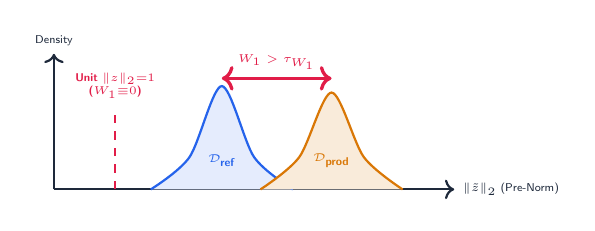
\begin{tikzpicture}[scale=0.82, every node/.style={transform shape}]
                    \draw[->, thick, SlateMid] (0,0) -- (6.2,0) node[right, font=\tiny] {$\|\tilde{z}\|_2$ (Pre-Norm)};
                    \draw[->, thick, SlateMid] (0,0) -- (0,2.1) node[above, font=\tiny] {Density};
                    \draw[dashed, RoseAccent, thick] (0.95,0) -- (0.95,1.28) node[above, font=\tiny\bfseries, align=flush center] {Unit $\|z\|_2{=}1$\\($W_1{\equiv}0$)};
                    % Reference curve
                    \draw[thick, BlueAccent, fill=BlueAccent!12] plot[smooth] coordinates {(1.5,0) (2.1,0.5) (2.6,1.60) (3.1,0.5) (3.7,0)};
                    \node[font=\tiny\bfseries\color{BlueAccent}] at (2.6, 0.45) {$\mathcal{D}_{\text{ref}}$};
                    % Drifted curve
                    \draw[thick, AmberAccent, fill=AmberAccent!15] plot[smooth] coordinates {(3.2,0) (3.8,0.5) (4.3,1.50) (4.8,0.5) (5.4,0)};
                    \node[font=\tiny\bfseries\color{AmberAccent}] at (4.3, 0.45) {$\mathcal{D}_{\text{prod}}$};
                    \draw[<->, very thick, RoseAccent] (2.6, 1.72) -- (4.3, 1.72) node[midway, above, font=\tiny\bfseries] {$W_1 > \tau_{W_1}$};
                \end{tikzpicture}%
                }
                \vspace{1pt}
                {\tiny Catches illumination, contrast \& sensor shifts in sub-millisecond time.}
            \end{tcolorbox}
        \end{column}
        \begin{column}{0.48\textwidth}
            \begin{tcolorbox}[enhanced, colback=white, colframe=TealAccent!60, boxrule=0.6pt, arc=2.5pt, left=4pt, right=4pt, top=2.5pt, bottom=2.5pt]
                \centering\textbf{\scriptsize\color{TealAccent} Tier 2: Unbiased RBF Kernel $\text{MMD}_u^2$ ($\mathcal{O}((M+N)^2 D)$)}\\[2pt]
                \resizebox{0.89\linewidth}{!}{%
                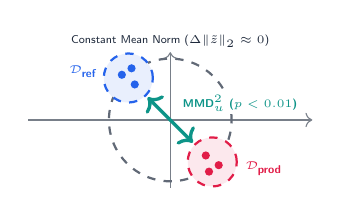
\begin{tikzpicture}[scale=0.82, every node/.style={transform shape}]
                    \draw[->, SlateMid!60] (-2.2,0) -- (2.2,0);
                    \draw[->, SlateMid!60] (0,-1.05) -- (0,1.05);
                    \draw[dashed, SlateMid!70, thick] (0,0) circle (0.95cm);
                    \node[font=\tiny\color{SlateMid}] at (0, 1.22) {Constant Mean Norm ($\Delta\|\tilde{z}\|_2 \approx 0$)};
                    % Cluster 1
                    \draw[dashed, BlueAccent, thick, fill=BlueAccent!10] (-0.65, 0.65) circle (0.38cm);
                    \fill[BlueAccent] (-0.75,0.7) circle (1.8pt) (-0.55,0.55) circle (1.8pt) (-0.6,0.8) circle (1.8pt);
                    \node[font=\tiny\bfseries\color{BlueAccent}] at (-1.35, 0.75) {$\mathcal{D}_{\text{ref}}$};
                    % Cluster 2 (rotated)
                    \draw[dashed, RoseAccent, thick, fill=RoseAccent!10] (0.65, -0.65) circle (0.38cm);
                    \fill[RoseAccent] (0.75,-0.7) circle (1.8pt) (0.55,-0.55) circle (1.8pt) (0.6,-0.8) circle (1.8pt);
                    \node[font=\tiny\bfseries\color{RoseAccent}] at (1.45, -0.75) {$\mathcal{D}_{\text{prod}}$};
                    \draw[<->, very thick, TealAccent] (-0.35, 0.35) -- (0.35, -0.35) node[midway, above right=2pt and 4pt, fill=white, inner sep=1pt, font=\tiny\bfseries] {$\text{MMD}_u^2$ ($p < 0.01$)};
                \end{tikzpicture}%
                }
                \vspace{1pt}
                {\tiny Permutation test ($B=200$) catches 384-D manifold rotations at fixed norm.}
            \end{tcolorbox}
        \end{column}
    \end{columns}
    \vspace{0.08cm}
    \begin{greencard}
        \centering
        \textbf{\color{GreenAccent} Async Pipeline:} \toollogo{fastapi}FastAPI logs \textbf{pre-normalised} $\tilde{z} \in \mathbb{R}^{384}$ via \texttt{BackgroundTasks} to \toollogo{postgresql}PostgreSQL ($\approx 1.5\text{ KB}$/row) $\to$ \toollogo{airflow}Airflow evaluates hourly against \texttt{cal\_embeddings.pt} $\to$ \toollogo{evidently}\textbf{Evidently 0.7 (\texttt{:30082})} renders 8 PCA + norm cards $\to$ logs HTML to \toollogo{dagshub}DagsHub \texttt{taxon-vision-drift}.
    \end{greencard}
    \note{
        \textbf{Time: 10:35-11:45 (1m 10s)}
        \begin{itemize}
            \item \textbf{Jury Question: How do you detect data drift or performance drift in production?}
            \item Notice a subtle mathematical pitfall: if you $L_2$-normalise embeddings onto the unit sphere prior to drift checks, every vector norm collapses to $1.0$, making 1D norm Wasserstein-1 blind ($|1 - 1| = 0$). That is why our ONNX graph outputs \textbf{pre-normalised} 384-D activations $\tilde{z}$, persisted asynchronously via \texttt{BackgroundTasks}.
            \item \textbf{Tier 1 (Panel A):} Fast $\mathcal{O}(N)$ 1D \textbf{Wasserstein-1 ($W_1$)} on pre-normalised norms ($\tau_{W_1} = 0.1281$ bootstrapped / $0.15$ config baseline) catches sensor, contrast, and lighting shifts immediately.
            \item \textbf{Tier 2 (Panel B):} If a seasonal species shift rotates the representation manifold at constant norm, $W_1$ misses it. Our unbiased RBF kernel \textbf{$\text{MMD}_u^2$} permutation test ($B=200$, $p < 0.01$) detects multivariate distribution shift across all 384 dimensions, whilst \textbf{Evidently 0.7} (\texttt{:30082}) projects 8 PCA columns + norms to DagsHub MLflow.
        \end{itemize}
    }
\end{frame}

% ==============================================================================
% SLIDE 11: Observability Cockpit & Closed-Loop Retraining (11:45 - 12:50)
% ==============================================================================
\begin{frame}{Observability \& Closed-Loop}{17-Panel Grafana, 6h Cooldown \& Triage}
    \centering
    \resizebox{0.94\textwidth}{!}{%
    \begin{tikzpicture}
        % Left: Sources
        \node[sysbox, draw=AmberAccent, fill=AmberAccent!10, text width=3.1cm] (src1) at (0, 1.45) {
            \textbf{\toollogo{prometheus}Prometheus (\texttt{:30090})}\\
            {\tiny Scrapes \texttt{/metrics} (15s)}\\
            {\tiny \texttt{DriftMetricsCollector} (30s TTL)}
        };
        \node[sysbox, draw=AmberAccent, fill=AmberAccent!10, text width=3.1cm] (src2) at (0, 0.10) {
            \textbf{Promtail $\to$ Loki 3.0}\\
            {\tiny Structured JSON Logs}\\
            {\tiny Pod / Endpoint Labels}
        };

        % Center-Left: Grafana 17 Panels
        \node[sysbox, draw=AmberAccent, fill=AmberAccent!18, text width=3.8cm] (graf) at (4.15, 0.75) {
            \textbf{\color{AmberAccent} \toollogo{grafana}Grafana Cockpit (\texttt{:30300})}\\
            {\tiny \textbf{Dashboard 1 (7 Panels):} Latency p50/p95/p99, $|\hat{C}|$, OOD Rate, $W_1$/$\text{MMD}^2$}\\
            {\tiny \textbf{Dashboard 2 (10 Panels):} GPU VRAM, CPU/RAM, NVMe, Loki Logs}
        };

        % Path A: Machine Retraining Loop (Top Right)
        \node[sysbox, draw=BlueAccent, fill=BlueAccent!12, text width=3.4cm] (hook) at (9.90, 1.55) {
            \textbf{\color{BlueAccent} \toollogo{fastapi}FastAPI Webhook Relay}\\
            {\tiny \texttt{POST /api/v1/retrain/webhook}}\\
            {\tiny Bearer Auth + \textbf{6h Cooldown Lock}}
        };
        \node[sysbox, draw=GreenAccent, fill=GreenAccent!12, text width=3.2cm] (air) at (13.75, 1.55) {
            \textbf{\color{GreenAccent} \toollogo{airflow}Airflow $\to$ \toollogo{jenkins}Jenkins GPU}\\
            {\tiny OAuth2 JWT $\to$ \texttt{model\_retraining}}\\
            {\tiny 8-Stage DVC + 4-Gate Check}
        };

        % Path B: Human Active Learning Loop (Bottom Right)
        \node[sysbox, draw=PurpleAccent, fill=PurpleAccent!12, text width=3.4cm] (ls) at (9.90, -0.15) {
            \textbf{\color{PurpleAccent} \toollogo{dagshub}DagsHub Label Studio}\\
            {\tiny Conformal / Energy Triage Queue}\\
            {\tiny Taxonomist + Forward CAM}
        };
        \node[sysbox, draw=TealAccent, fill=TealAccent!12, text width=3.2cm] (mrg) at (13.75, -0.15) {
            \textbf{\color{TealAccent} Manifest Expansion}\\
            {\tiny \texttt{merge\_human\_feedback}}\\
            {\tiny Validates CC Licence $\to$ DVC}
        };

        \draw[flowarrow] (src1.east) -- ++(0.25,0) |- (graf.west);
        \draw[flowarrow] (src2.east) -- ++(0.25,0) |- (graf.west);
        \draw[retrainarrow] (graf.east) -- ++(0.35,0) |- (hook.west);
        \node[font=\tiny\bfseries\color{RoseAccent}, above=2pt] at (7.30, 1.55) {Path A: Alert};
        \draw[flowarrow] (hook) -- (air);
        \draw[flowarrow, draw=PurpleAccent] (graf.east) -- ++(0.35,0) |- (ls.west);
        \node[font=\tiny\bfseries\color{PurpleAccent}, below=2pt] at (7.30, -0.15) {Path B: Triage};
        \draw[flowarrow] (ls) -- (mrg);
        \draw[passarrow] (mrg.north) -- (air.south);
    \end{tikzpicture}%
    }
    \vspace{0.15cm}
    \begin{bluecard}
        \centering
        \textbf{\color{BlueAccent} Four Alert Rules \& Anti-Storm Lock:} \texttt{PredictionLatencyP95High} ($>350\text{ ms}$), \texttt{PredictionErrorRatioHigh} ($>5\%$), \texttt{DriftMonitorStale} ($>2\text{h}$), and \texttt{EmbeddingDriftDetected} (\texttt{taxon\_drift\_detected} $> 0.5$ $\to$ \texttt{action=retrain} guarded by an atomic \textbf{6h cooldown} \texttt{21600s}).
    \end{bluecard}
    \note{
        \textbf{Time: 11:45-12:50 (1m 05s)}
        \begin{itemize}
            \item \textbf{Jury Questions: Which indicators are monitored in Grafana and where do they come from? Do drifts trigger an alert, retraining, or manual review?}
            \item Grafana (\texttt{:30300}) renders \textbf{17 visual panels across 2 provisioned dashboards}: 7 MLOps panels fed by Prometheus scraping \texttt{/metrics} every 15s (p50/p95/p99 latency, status counts, conformal referrals, and persistent PostgreSQL drift gauges via \texttt{DriftMetricsCollector}) plus 10 infrastructure and Loki 3.0 log panels (node CPU/RAM, 4-slot GPU VRAM, Promtail JSON logs).
            \item Drift is integrated via a \textbf{bifurcated closed loop} - alert + automatic retraining + human review:
            \item \textbf{Path A (Automated Retraining):} \texttt{EmbeddingDriftDetected} notifies \texttt{POST /api/v1/retrain/webhook} (constant-time Bearer auth). FastAPI acquires an atomic \textbf{6-hour cooldown lock} to stop alert storms, fetches an Airflow OAuth2 JWT, and triggers \texttt{model\_retraining}.
            \item \textbf{Path B (Human Review):} OOD and ambiguous observations queue in \texttt{TriageQueue} for taxonomist audit (Conformal/Energy gating + Forward CAM) and re-enter \texttt{raw\_manifest.parquet} after open-licence verification.
        \end{itemize}
    }
\end{frame}

% ==============================================================================
% SLIDE 12: Four-Gate Promotion, Docker Isolation & Security (12:50 - 13:55)
% ==============================================================================
\begin{frame}{Quality Gates, Docker \& Security}{4-Gate Promotion, Non-Root Images \& k3s}
    \begin{columns}[T]
        \begin{column}{0.48\textwidth}
            \centering
            \textbf{\scriptsize\color{GreenAccent} Stage 8 Four-Gate Verdict (\texttt{promotion.py})}\\[3pt]
            \resizebox{\textwidth}{!}{%
            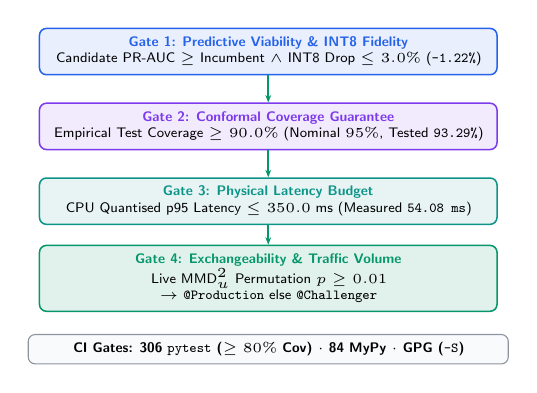
\begin{tikzpicture}
                \node[sysbox, draw=BlueAccent, fill=BlueAccent!10, text width=5.6cm] (g1) at (0, 2.1) {
                    \textbf{\color{BlueAccent} Gate 1: Predictive Viability \& INT8 Fidelity}\\
                    {\tiny Candidate PR-AUC $\ge$ Incumbent $\wedge$ INT8 Drop $\le 3.0\%$ (\texttt{-1.22\%})}
                };
                \node[sysbox, draw=PurpleAccent, fill=PurpleAccent!10, text width=5.6cm] (g2) at (0, 1.15) {
                    \textbf{\color{PurpleAccent} Gate 2: Conformal Coverage Guarantee}\\
                    {\tiny Empirical Test Coverage $\ge 90.0\%$ (Nominal $95\%$, Tested \texttt{93.29\%})}
                };
                \node[sysbox, draw=TealAccent, fill=TealAccent!10, text width=5.6cm] (g3) at (0, 0.20) {
                    \textbf{\color{TealAccent} Gate 3: Physical Latency Budget}\\
                    {\tiny CPU Quantised p95 Latency $\le 350.0\text{ ms}$ (Measured \texttt{54.08 ms})}
                };
                \node[sysbox, draw=GreenAccent, fill=GreenAccent!12, text width=5.6cm] (g4) at (0, -0.78) {
                    \textbf{\color{GreenAccent} Gate 4: Exchangeability \& Traffic Volume}\\
                    {\tiny Live $\text{MMD}_u^2$ Permutation $p \ge 0.01$}\\
                    {\tiny $\to$ \texttt{@Production} else \texttt{@Challenger}}
                };
                \node[pill, fill=SlateLight, draw=SlateMid!50, text width=5.9cm] (tst) at (0, -1.68) {
                    \textbf{CI Gates: 306 \texttt{pytest} ($\ge 80\%$ Cov)} $\cdot$ 84 MyPy $\cdot$ GPG (\texttt{-S})
                };
                \draw[passarrow] (g1) -- (g2);
                \draw[passarrow] (g2) -- (g3);
                \draw[passarrow] (g3) -- (g4);
            \end{tikzpicture}%
            }
        \end{column}
        \begin{column}{0.48\textwidth}
            \centering
            \textbf{\scriptsize\color{RoseAccent} \toollogo{docker}Docker Purpose \& \toollogo{kubernetes}K3s Security Posture}\\[3pt]
            \resizebox{\textwidth}{!}{%
            \begin{tikzpicture}
                \node[sysbox, draw=BlueAccent, fill=BlueAccent!10, text width=5.6cm] (s1) at (0, 2.1) {
                    \textbf{\color{BlueAccent} \toollogo{docker}1. Multi-Stage Non-Root Docker Isolation}\\
                    {\tiny Locks \texttt{pixi.lock} + ONNX/CUDA across CI \& K3s}\\
                    {\tiny Non-root UIDs: \texttt{10001}, \texttt{50000}, \texttt{70}}
                };
                \node[sysbox, draw=SlateDark, fill=SlateLight, text width=5.6cm] (s2) at (0, 1.15) {
                    \textbf{2. Zero Inbound Ports \& Scoped RBAC}\\
                    {\tiny Outbound Cloudflare Tunnel + Namespace \texttt{jenkins-deployer-role}}
                };
                \node[sysbox, draw=RoseAccent, fill=RoseAccent!10, text width=5.6cm] (s3) at (0, 0.20) {
                    \textbf{\color{RoseAccent} 3. Constant-Time Bearer, JWT \& Trap Cleanup}\\
                    {\tiny \texttt{INTERNAL\_API\_TOKEN} $\cdot$ \texttt{RETRAIN\_WEBHOOK\_SECRET} $\cdot$ \texttt{EXIT} DVC Scrub}
                };
                \node[sysbox, draw=AmberAccent, fill=AmberAccent!12, text width=5.6cm] (s4) at (0, -0.85) {
                    \textbf{\color{AmberAccent} 4. Out-of-Band Secrets \& Hardening Roadmap}\\
                    {\tiny \textbf{Active:} Non-root containers + \texttt{0600} stdin secrets (\texttt{kubectl apply -f -})}\\
                    {\tiny \textbf{Next:} FluxCD + SOPS/\texttt{age}, Traefik Rate-Limit/OIDC, \texttt{NetworkPolicy}}
                };
                \draw[flowarrow] (s1) -- (s2);
                \draw[flowarrow] (s2) -- (s3);
                \draw[flowarrow] (s3) -- (s4);
            \end{tikzpicture}%
            }
        \end{column}
    \end{columns}

    \note{
        \textbf{Time: 12:50-13:55 (1m 05s)}
        \begin{itemize}
            \item \textbf{Jury Questions: How do you evaluate model robustness before production? What is the purpose of Docker? How do you manage API security and how can it be improved?}
            \item \textbf{Pre-Deployment Robustness:} Stage 8 enforces our sequential Four-Gate check in \texttt{promotion.py}: (1) PR-AUC $\ge$ incumbent and INT8 drop $\le 3\%$, (2) test coverage $\ge 90\%$, (3) CPU p95 $\le 350\text{ ms}$, and (4) live $\text{MMD}_u^2$ $p \ge 0.01$. Code integrity is backed by \textbf{306 pytest cases}, strict MyPy across \textbf{84 files}, \texttt{complexipy} ($< 15$), OKF validation, and mandatory GPG-signed commits.
            \item \textbf{Docker:} Eliminates environment drift across laptop, GitHub Actions, Jenkins, and K3s by compiling locked \texttt{pixi.lock} + CUDA 12.8 dependencies into minimal non-root images (FastAPI UID \texttt{10001}, Airflow \texttt{50000}, Postgres \texttt{70}).
            \item \textbf{Security \& Next Steps:} Zero open router ports (Cloudflare Tunnel), fail-closed constant-time Bearer tokens on \texttt{/drift/evaluate} and \texttt{/retrain/webhook}, Airflow OAuth2 JWT, Jenkins \texttt{EXIT} trap credential cleanup, and out-of-band K3s Secrets via \texttt{0600} \texttt{stdin}. Next hardening phase: FluxCD + SOPS/\texttt{age}, Traefik rate limiting + OIDC on public routes, and K8s \texttt{NetworkPolicy}/mTLS.
        \end{itemize}
    }
\end{frame}

% ==============================================================================
% SLIDE 13: 5-Minute Live Demonstration Walkthrough (13:55 - 14:30)
% ==============================================================================
\begin{frame}{Live Cluster Demo (5 Minutes)}{Walkthrough Across Live k3s \& DagsHub}
    \centering
    \vspace{0.1cm}
    \resizebox{0.98\textwidth}{!}{%
    \begin{tikzpicture}
        \node[sysbox, draw=GreenAccent, fill=GreenAccent!10, text width=3.80cm, minimum height=2.45cm] (d1) at (0, 0) {
            \textbf{\color{GreenAccent} Step 1 (0:00-1:30)}\\
            \textbf{\toollogo{fastapi}HTMX Cockpit \& \toollogo{redis}CAM}\\[2pt]
            {\tiny \texttt{taxon.benjamin-foerster.eu}}\\
            {\tiny \texttt{taxon-staging.benjamin-foerster.eu}}\\[3pt]
            {\tiny \textbullet\ Live INT8 ONNX Prediction}\\
            {\tiny \textbullet\ Conformal $C(x)$ \& Energy Badge}\\
            {\tiny \textbullet\ On-Demand CAM via Redis}
        };
        \node[sysbox, draw=AmberAccent, fill=AmberAccent!10, text width=3.80cm, minimum height=2.45cm] (d2) at (4.25, 0) {
            \textbf{\color{AmberAccent} Step 2 (1:30-2:45)}\\
            \textbf{\toollogo{grafana}Grafana \& \toollogo{evidently}Evidently}\\[2pt]
            {\tiny \texttt{taxon-grafana.benjamin-foerster.eu}}\\
            {\tiny \texttt{taxon-evidently.benjamin-foerster.eu}}\\[3pt]
            {\tiny \textbullet\ 17 Panels (MLOps + Infra)}\\
            {\tiny \textbullet\ Loki 3.0 Structured Logs}\\
            {\tiny \textbullet\ $W_1$ \& PCA Drift Cards}
        };
        \node[sysbox, draw=BlueAccent, fill=BlueAccent!10, text width=3.80cm, minimum height=2.45cm] (d3) at (8.50, 0) {
            \textbf{\color{BlueAccent} Step 3 (2:45-4:00)}\\
            \textbf{\toollogo{dagshub}DagsHub \& \toollogo{optuna}Optuna}\\[2pt]
            {\tiny \texttt{dagshub.com/foersben/...}}\\
            {\tiny \texttt{taxon-optuna.benjamin-foerster.eu}}\\[3pt]
            {\tiny \textbullet\ 8-Stage DVC Lineage Graph}\\
            {\tiny \textbullet\ \toollogo{mlflow}MLflow 3.x Parent Run \& Plots}\\
            {\tiny \textbullet\ \texttt{@Production} + Passports}
        };
        \node[sysbox, draw=PurpleAccent, fill=PurpleAccent!10, text width=3.80cm, minimum height=2.45cm] (d4) at (12.75, 0) {
            \textbf{\color{PurpleAccent} Step 4 (4:00-5:00)}\\
            \textbf{\toollogo{airflow}Airflow 3 \& \toollogo{jenkins}Jenkins}\\[2pt]
            {\tiny \texttt{taxon-airflow.benjamin-foerster.eu}}\\
            {\tiny \texttt{jenkins.benjamin-foerster.eu}}\\[3pt]
            {\tiny \textbullet\ \texttt{prediction\_drift\_monitor}}\\
            {\tiny \textbullet\ \texttt{model\_retraining} TaskFlow}\\
            {\tiny \textbullet\ 7-Stage RTX 5070 Ti Build}
        };

        \draw[passarrow] (d1) -- (d2);
        \draw[passarrow] (d2) -- (d3);
        \draw[passarrow] (d3) -- (d4);
    \end{tikzpicture}%
    }
    \vspace{0.35cm}
    \begin{tcolorbox}[enhanced, width=0.80\textwidth, colback=SlateDark, colframe=BlueAccent, boxrule=0.6pt, arc=3pt, top=4pt, bottom=4pt]
        \centering\footnotesize\color{white}
        \textbf{Live Demo Walkthrough:} 5-minute tour across the cluster tabs before closing conclusions \& jury Q\&A.
    \end{tcolorbox}
    \note{
        \textbf{Time: 13:55-14:30 (35s) $\to$ Transition to 5-Min Live Demo}
        \begin{itemize}
            \item That concludes the 15-minute architecture walk-through. I will now move to the live cluster across four tabs:
            \item \textbf{1.} \texttt{taxon.benjamin-foerster.eu} \& \texttt{taxon-staging.benjamin-foerster.eu} - submit an in-distribution bird/insect photo for conformal set + CAM, plus an OOD image for triage routing.
            \item \textbf{2.} \texttt{taxon-grafana.benjamin-foerster.eu} \& \texttt{taxon-evidently.benjamin-foerster.eu} - show live scraped request metrics, Loki logs, and $W_1$/PCA drift diagnostics.
            \item \textbf{3.} \texttt{dagshub.com/foersben/taxon-vision-mlops} \& \texttt{taxon-optuna.benjamin-foerster.eu} - show the 8-stage DVC lineage, MLflow parent run, and Optuna Postgres trials.
            \item \textbf{4.} \texttt{taxon-airflow.benjamin-foerster.eu} \& \texttt{jenkins.benjamin-foerster.eu} - show both TaskFlow DAGs and a green 7-stage GPU deployment.
        \end{itemize}
    }
\end{frame}

% ==============================================================================
% SLIDE 15: Project Conclusion & Next Steps (Post-Demo Closing & Q&A Anchor)
% ==============================================================================
\begin{frame}{Conclusion \& Next Steps}{Proven Production Chain \& Closing Loop Gaps}
    \begin{columns}[c]
        \begin{column}{0.48\textwidth}
            \begin{greencard}
                \textbf{\color{GreenAccent} Project Conclusion: What Is Proven Live}\\[3pt]
                \textbullet\ \textbf{Fast, Reproducible Serving:} \toollogo{onnx}\textbf{INT8 ONNX} via \toollogo{fastapi}\textbf{FastAPI} on \toollogo{kubernetes}\textbf{k3s} delivers \textbf{54.08 ms p95} CPU latency ($91.46\%$ accuracy) with pre-warmed startup singletons.\\[3pt]
                \textbullet\ \textbf{Mathematically Bounded Safety:} Split Conformal sets ($95\%$ target, $93.29\%$ tested) and Helmholtz OOD gating route unfamiliar specimens to human triage.\\[3pt]
                \textbullet\ \textbf{Automated Lineage \& Healing:} \toollogo{dvc}\textbf{8-stage DVC} + \toollogo{mlflow}\textbf{MLflow 4-gate} promotion + \toollogo{grafana}\textbf{Grafana}/\toollogo{evidently}\textbf{Evidently} drift $\to$ \toollogo{airflow}\textbf{Airflow} $\to$ \toollogo{jenkins}\textbf{Jenkins} GPU retraining.
            \end{greencard}
        \end{column}
        \begin{column}{0.49\textwidth}
            \begin{bluecard}
                \textbf{\color{BlueAccent} Next Steps: Closing Remaining Loop Gaps}\\[3pt]
                \textbullet\ \textbf{1. Active Learning Diversity (\texttt{BADGE} / \texttt{k-means++}):} Currently \texttt{TriageQueue} uses Conformal/Energy gating and \texttt{query.py} implements margin sampling only; wire batch-diverse \texttt{BADGE}/\texttt{k-means++} selection before \toollogo{dagshub}\textbf{Label Studio} upload.\\[3pt]
                \textbullet\ \textbf{2. Pipeline 2 (\texttt{LanceDB HNSW} + KG) \& Routing:} Add $\mathcal{O}(1)$ taxonomic splits/lumps without retraining and an automated router deciding Pipeline 1 retraining vs.\ Pipeline 2 index updates.\\[3pt]
                \textbullet\ \textbf{3. GitOps, Security \& Scaling:} Migrate to \texttt{FluxCD + SOPS/age}, add Traefik rate-limit/OIDC, \texttt{NetworkPolicy}/mTLS, and K8s \texttt{HPA}.
            \end{bluecard}
        \end{column}
    \end{columns}
    \vspace{0.18cm}
    \centering
    \begin{tcolorbox}[enhanced, width=0.82\textwidth, colback=SlateDark, colframe=BlueAccent, boxrule=0.6pt, arc=3pt, top=4pt, bottom=4pt]
        \centering\footnotesize\color{white}
        \textbf{Thank you for your attention!} $\cdot$ Ready for Jury Q\&A
    \end{tcolorbox}
    \note{
        \textbf{Post-Demo Closing Slide (Leave up during Jury Q\&A)}
        \begin{itemize}
            \item \textbf{Conclusion:} TaxonVision-MLOps delivers the complete production chain requested in the project brief - open-licensed AWS data, frozen DINOv3 + INT8 ONNX serving at 54 ms p95, conformal uncertainty with human triage, and automated drift-triggered GPU retraining.
            \item \textbf{Honest Next Steps:} (1) wire true batch-diverse \texttt{BADGE}/\texttt{k-means++} selection into \texttt{TriageQueue} ahead of Label Studio (today it queues by Conformal/Energy boundaries whilst \texttt{query.py} implements margin sampling), (2) implement Pipeline 2 (\texttt{LanceDB HNSW} + knowledge graph) with a decision gate choosing index updates vs.\ weight retraining, and (3) complete declarative \texttt{FluxCD + SOPS/age} GitOps, Traefik rate-limiting/OIDC, \texttt{NetworkPolicy}/mTLS, and multi-node K8s \texttt{HPA}.
        \end{itemize}
    }
\end{frame}

% ==============================================================================
% BACKUP SLIDE B1: Traffic Spikes & Resource Budgeting (For Q&A)
% ==============================================================================
\begin{frame}{Backup B1: Traffic Burst Scaling}{Async Offloading, Thread Caps \& K8s HPA}
    \centering
    \resizebox{0.97\textwidth}{!}{%
    \begin{tikzpicture}
        \node[sysbox, draw=BlueAccent, fill=BlueAccent!10, text width=3.95cm] (b1) at (0, 0) {
            \textbf{\color{BlueAccent} \toollogo{fastapi}1. Non-Blocking Event Loop}\\
            {\tiny \texttt{anyio.to\_thread.run\_sync} for ONNX}\\
            {\tiny \texttt{BackgroundTasks} for Postgres / S3}
        };
        \node[sysbox, draw=TealAccent, fill=TealAccent!10, text width=4.05cm] (b2) at (4.85, 0) {
            \textbf{\color{TealAccent} \toollogo{kubernetes}2. Active 2-Replica Pool}\\
            {\tiny \texttt{maxSurge=1, maxUnavailable=0}}\\
            {\tiny \texttt{intra\_op\_threads=2} $\cdot$ \texttt{200m-2} CPU / \texttt{1-4 GiB}}
        };
        \node[sysbox, draw=GreenAccent, fill=GreenAccent!12, text width=4.15cm] (b3) at (9.80, 0) {
            \textbf{\color{GreenAccent} \toollogo{prometheus}3. Elastic HPA (Next-Phase)}\\
            {\tiny Prometheus Adapter $\to$ \textbf{K8s HPA}}\\
            {\tiny Triggers on p95 Latency \& Queue Depth}
        };
        \draw[flowarrow] (b1) -- (b2);
        \draw[passarrow] (b2) -- (b3);
    \end{tikzpicture}%
    }
    \vspace{0.18cm}
    \begin{columns}[T]
        \begin{column}{0.48\textwidth}
            \begin{bluecard}
                \raggedright
                \textbf{\color{BlueAccent} Active Single-Node Spike Resilience}\\[3pt]
                \textbullet\ \textbf{Bounded ONNX Concurrency:} \texttt{onnx\_intra\_op\_threads=2} prevents OpenMP thread oversubscription and CPU cgroup throttling inside containers.\\[2pt]
                \textbullet\ \textbf{Pre-Warmed Startup Singletons:} \texttt{@lru\_cache} model hydration avoids cold-start traffic storms during rolling surge pods.\\[2pt]
                \textbullet\ \textbf{Dedicated Staging Cap:} Staging uses \texttt{0} GPU slices so PR traffic never starves production or Jenkins builds.
            \end{bluecard}
        \end{column}
        \begin{column}{0.48\textwidth}
            \begin{greencard}
                \raggedright
                \textbf{\color{GreenAccent} Elastic Autoscaling \& Hardware Envelopes}\\[3pt]
                \textbullet\ \textbf{Primary Kubernetes Tool:} \textbf{HorizontalPodAutoscaler (HPA)} paired with Prometheus Adapter.\\[2pt]
                \textbullet\ \textbf{Latency-Driven Signal:} Scales directly on \texttt{taxon\_inference\_latency\_seconds} p95 rather than naive CPU utilisation alone.\\[2pt]
                \textbullet\ \textbf{VRAM Partitioning (16 GB RTX 5070 Ti):} 4 time-sliced virtual slots; training caps CUDA at $f=0.7$ ($11.2\text{ GB}$), preserving $4.8\text{ GB}$ headroom.
            \end{greencard}
        \end{column}
    \end{columns}

    \note{
        \cuetime{Backup B1}
        \cuejury{What happens if there is a traffic spike? Which tool is useful?}
        \begin{itemize}
            \item First, on our current cluster node, bursts do not stall FastAPI's event loop: two serving pods (\texttt{maxSurge=1, maxUnavailable=0}, \texttt{200m-2} CPU and \texttt{1-4 GiB} RAM) cap ONNX intra-op threads at \texttt{2} to prevent cgroup contention, offload CPU inference/drift math via \texttt{anyio.to\_thread.run\_sync}, and defer Postgres/S3 writes to \texttt{BackgroundTasks}.
            \item Second, for multi-node elastic burst scaling, the standard Kubernetes tool is the \textbf{HorizontalPodAutoscaler (HPA)} paired with \textbf{Prometheus Adapter}, scaling pods on custom SLO metrics such as \texttt{taxon\_inference\_latency\_seconds} p95 (with \textbf{KEDA} as a natural extension if asynchronous message-queue batch scoring is added).
            \item Meanwhile, GPU time-slicing exposes 4 virtual GPU slots whilst Stage 5 training enforces \texttt{TAXON\_CUDA\_MEMORY\_FRACTION=0.7} ($11.2\text{ GB}$ of $16\text{ GB}$) so training pods never starve active inference headroom.
        \end{itemize}
        \cueterms{\textbf{GPU Time-Slicing:} Sharing 1 physical GPU (\texttt{replicas: 4} virtual K8s slots) across pods by switching compute cycles; paired with \texttt{0.7} VRAM cap (\texttt{11.2 GB}) since memory is not hardware-isolated. $\cdot$ \textbf{HPA:} Horizontal Pod Autoscaler. $\cdot$ \textbf{KEDA:} Kubernetes Event-driven Autoscaling. $\cdot$ \textbf{cgroup:} Linux Control Group.}
    }
\end{frame}

% ==============================================================================
% BACKUP SLIDE B2: 6-Tier Testing & Code Invariants (For Q&A)
% ==============================================================================
\begin{frame}{Backup B2: 6-Tier Test Matrix}{306 Pytest Cases, Conformal Bounds \& AST}
    \centering
    \resizebox{0.97\textwidth}{!}{%
    \begin{tikzpicture}
        \node[sysbox, draw=BlueAccent, fill=BlueAccent!10, text width=3.9cm] (t1) at (0, 1.25) {
            \textbf{\color{BlueAccent} Tier 1: Upstream API Mocking}\\
            {\tiny \texttt{responses} intercepts iNaturalist}\\
            {\tiny HTTP 200, 429 backoff \& timeouts}
        };
        \node[sysbox, draw=TealAccent, fill=TealAccent!10, text width=3.9cm] (t2) at (4.45, 1.25) {
            \textbf{\color{TealAccent} \toollogo{dvc}Tier 2: S3 / DVC Mocking}\\
            {\tiny \texttt{moto} ephemeral in-memory S3}\\
            {\tiny Streaming, SigV4 \& hash integrity}
        };
        \node[sysbox, draw=PurpleAccent, fill=PurpleAccent!10, text width=3.9cm] (t3) at (8.90, 1.25) {
            \textbf{\color{PurpleAccent} Tier 3: Math \& Hardware Bounds}\\
            {\tiny Coverage $\frac{1}{n}\sum \mathbb{I}(y_i \in C(x_i)) \ge 1-\alpha$}\\
            {\tiny Enforces hardware spec invariants}
        };
        \node[sysbox, draw=AmberAccent, fill=AmberAccent!10, text width=3.9cm] (t4) at (0, -0.25) {
            \textbf{\color{AmberAccent} \toollogo{fastapi}Tier 4: Serving \& Auth Routes}\\
            {\tiny FastAPI integration (\texttt{/predict}, \texttt{/drift})}\\
            {\tiny Constant-time Bearer \& 6h cooldown}
        };
        \node[sysbox, draw=RoseAccent, fill=RoseAccent!10, text width=3.9cm] (t5) at (4.45, -0.25) {
            \textbf{\color{RoseAccent} Tier 5: Static \& AST Governance}\\
            {\tiny 84 MyPy strict files $\cdot$ \texttt{complexipy} $<15$}\\
            {\tiny Ruff lint $\cdot$ OKF v0.2 $\cdot$ Licence gate}
        };
        \node[sysbox, draw=GreenAccent, fill=GreenAccent!10, text width=3.9cm] (t6) at (8.90, -0.25) {
            \textbf{\color{GreenAccent} Tier 6: Live Cluster Smoke Probe}\\
            {\tiny \texttt{verify\_deployment.sh} post-rollout}\\
            {\tiny Probes \texttt{/health}, \texttt{/health/ready}, \texttt{/metrics}}
        };
    \end{tikzpicture}%
    }
    \vspace{0.22cm}
    \begin{bluecard}
        \centering
        \textbf{\color{BlueAccent} Continuous Enforcement:} \toollogo{githubactions}GitHub Actions (\texttt{ci-dev} CPU matrix) \& \toollogo{jenkins}Jenkins Stage 2-4 enforce all \textbf{306 collected \texttt{pytest} tests} with an \textbf{$\ge 80\%$ line-coverage gate} (\texttt{--cov-fail-under=80}), followed post-rollout by Tier 6 live cluster smoke probes (\texttt{/api/v1/predict} \& \toollogo{prometheus}Prometheus metrics).
    \end{bluecard}
    \note{
        \textbf{Backup B2 - Q\&A: Which unit tests have been implemented and what are they used for?}
        \begin{itemize}
            \item We enforce \textbf{306 collected \texttt{pytest} cases} across unit, integration, and invariant suites with a strict \textbf{80\% CI coverage floor} (\texttt{--cov-fail-under=80}), organised across six complementary verification tiers:
            \item \textbf{(1) HTTP Mocking (\texttt{responses}):} Verifies iNaturalist ingestion pagination, HTTP 429 exponential backoff, and timeout resilience without hitting upstream rate limits.
            \item \textbf{(2) S3 Mocking (\texttt{moto}):} Tests zero-tarball S3 streaming, SigV4 authentication, and triage queue uploads purely in RAM.
            \item \textbf{(3) Mathematical \& Hardware Invariants:} Verifies Split Conformal coverage ($\ge 1 - \alpha$) mathematically, finite-sample quantile bounds, and Rule 07 hardware parameter checks.
            \item \textbf{(4) Integration Routes \& Security:} Exercises FastAPI \texttt{/api/v1/predict}, \texttt{/drift/evaluate}, and \texttt{/retrain/webhook}, validating fail-closed 503/401 Bearer checks and atomic 6h cooldown locking.
            \item \textbf{(5) Static \& Governance Gates:} MyPy across 84 source files, Ruff, \texttt{complexipy} ($<15$), OKF frontmatter validation, and Creative Commons licence audits.
            \item \textbf{(6) Live Cluster Smoke Probe:} \texttt{verify\_deployment.sh} validates rollout convergence, \texttt{/health}, \texttt{/health/ready}, \texttt{POST /api/v1/predict}, and Prometheus \texttt{taxon\_predictions\_total} after every Jenkins deployment.
        \end{itemize}
    }
\end{frame}

% ==============================================================================
% BACKUP SLIDE B3: API Security & Hardening Roadmap (For Q&A)
% ==============================================================================
\begin{frame}{Backup B3: Security \& Hardening}{Zero-Trust Controls \& Next-Phase Roadmap}
    \begin{columns}[c]
        \begin{column}{0.51\textwidth}
            \centering
            \resizebox{\textwidth}{!}{%
            \begin{tikzpicture}
                \node[sysbox, draw=GreenAccent, fill=GreenAccent!10, text width=5.6cm] (sec1) at (0, 2.10) {
                    \textbf{\color{GreenAccent} 1. Zero-Port Edge \& Scoped RBAC}\\
                    {\tiny Outbound Cloudflare \texttt{hive-mind-tunnel} $\cdot$ Namespace \texttt{jenkins-deployer-role}}
                };
                \node[sysbox, draw=BlueAccent, fill=BlueAccent!10, text width=5.6cm] (sec2) at (0, 1.05) {
                    \textbf{\color{BlueAccent} 2. Fail-Closed Bearer Auth (503 / 401)}\\
                    {\tiny \texttt{hmac.compare\_digest} on \texttt{/drift/evaluate} \& \texttt{/retrain/webhook}}
                };
                \node[sysbox, draw=PurpleAccent, fill=PurpleAccent!10, text width=5.6cm] (sec3) at (0, 0.0) {
                    \textbf{\color{PurpleAccent} 3. Control-Plane JWT, CSRF \& Key Scrubbing}\\
                    {\tiny \toollogo{airflow}Airflow OAuth2 JWT $\cdot$ \toollogo{jenkins}Jenkins CSRF Crumb $\cdot$ \texttt{EXIT} DVC key cleanup}
                };
                \node[sysbox, draw=TealAccent, fill=TealAccent!10, text width=5.6cm] (sec4) at (0, -1.05) {
                    \textbf{\color{TealAccent} 4. Non-Root Runtime \& Out-of-Band Secrets}\\
                    {\tiny UIDs \texttt{10001}, \texttt{50000}, \texttt{70} $\cdot$ \texttt{0600} env file + \texttt{stdin} \texttt{kubectl apply -f -}}
                };
                \draw[flowarrow] (sec1) -- (sec2);
                \draw[flowarrow] (sec2) -- (sec3);
                \draw[flowarrow] (sec3) -- (sec4);
            \end{tikzpicture}%
            }
        \end{column}
        \begin{column}{0.46\textwidth}
            \begin{ambercard}
                \raggedright
                \textbf{\color{AmberAccent} How API Security Can Be Improved}\\[4pt]
                \textbullet\ \textbf{1. FluxCD + SOPS/\texttt{age} GitOps:} Replace imperative \texttt{provision\_k8s\_secrets.sh} with age-encrypted declarative GitOps secrets.\\[4pt]
                \textbullet\ \textbf{2. Public Route Rate-Limiting \& OIDC:} Enforce Traefik token-bucket rate limits and Cloudflare Access / OIDC JWT verification on \texttt{/predict}.\\[4pt]
                \textbullet\ \textbf{3. East-West mTLS \& \texttt{NetworkPolicy}:} Enforce default-deny Kubernetes \texttt{NetworkPolicy} rules between namespaces plus pod-to-pod mTLS.
            \end{ambercard}
        \end{column}
    \end{columns}

    \note{
        \textbf{Backup B3 - Q\&A: How do you manage API security, and how can it be improved?}
        \begin{itemize}
            \item \textbf{Active zero-trust posture:} No router ports are exposed externally - all ingress traverses an outbound Cloudflare Tunnel (\texttt{hive-mind-tunnel}). Control-plane mutations (\texttt{/api/v1/drift/evaluate} and \texttt{/api/v1/retrain/webhook}) fail closed with HTTP 503 if unconfigured or HTTP 401 on timing-safe \texttt{hmac.compare\_digest} mismatch.
            \item \textbf{Automation hygiene:} Airflow uses OAuth2 JWT tokens, Jenkins uses CSRF crumbs plus an \texttt{EXIT} trap scrubbing temporary DVC keys, containers drop to non-root UIDs (\texttt{10001}, \texttt{50000}, \texttt{70}), and secrets are provisioned out-of-band from a \texttt{0600} env file piped via \texttt{stdin} to \texttt{kubectl apply -f -}.
            \item \textbf{Concrete next-phase improvements:} (1) migrating secret provisioning to declarative \textbf{FluxCD + SOPS/\texttt{age}} GitOps (already noted as the target in \texttt{provision\_k8s\_secrets.sh}), (2) adding Traefik rate-limiting middleware and OIDC authentication on public inference routes, and (3) enforcing Kubernetes \texttt{NetworkPolicy} isolation plus East-West mTLS.
        \end{itemize}
    }
\end{frame}

\end{document}
